\documentclass[compress]{beamer}
\usetheme{CambridgeUS}
\useinnertheme{rounded}
\useoutertheme{miniframes}
%\usebeamercolor{lily}
%\useoutertheme{infolines}
\usepackage{graphicx}
\usepackage{setspace}
\usepackage{tabularx}
\usepackage[italian]{babel}
\usepackage{tikzsymbols}
\usepackage{tikz}
\usepackage{spot}
\usepackage{tabularx}
\usepackage[absolute,overlay]{textpos}
\usepackage{booktabs}
\usepackage{tikz}
\usepackage{xcolor}
\usepackage[utf8]{inputenc}
\definecolor{royalblue3}{RGB}{58,95,205}
\definecolor{giallo}{RGB}{197, 151, 0}
\definecolor{blu}{RGB}{19 101 158}
\usepackage[backend=biber, style=authoryear]{biblatex}
\setbeamertemplate{caption}[numbered]
%\addbibresource{biblio.bib}
\usetikzlibrary{mindmap,calc,patterns,decorations.pathmorphing,decorations.markings, arrows, shapes.arrows, shapes, backgrounds,positioning,shadows.blur}
%\usetikzlibrary{arrows,shapes}
\usepackage[absolute,overlay]{textpos}
\usetikzlibrary{shapes.geometric, arrows}
\tikzstyle{latent} = [ellipse, minimum width=2.5cm, minimum height=2cm,text centered, draw=black]
\tikzstyle{item} = [rectangle, rounded corners, minimum width=0.5cm, minimum height=2cm, text width =1.7cm, text centered, draw=black]
\tikzstyle{arrow} = [thick,->,>=stealth]

\definecolor{unipd}{RGB}{155, 0, 20}
\definecolor{grigioPantano}{RGB}{72,79,89}
\definecolor{blu}{rgb}{0.0, 0.33, 0.71}
\setbeamercolor{subsection name}{fg=white}
\setbeamercolor{section name}{fg=white}
\setbeamerfont{section title}{family=\bfseries}
\setbeamerfont{subsection title}{family=\bfseries}
\setbeamercolor{section title}{fg=template}

\def\tikzoverlay{%
	\tikz[remember picture, overlay]\node[every overlay node]
}%


\newcommand\Factor{1.2}


\AtBeginSection{\frame{\sectionpage}}
\setbeamertemplate{subsection page}
{
	\begingroup
	\begin{beamercolorbox}[sep=12pt,center]{section title}
		\usebeamerfont{section title}\insertsection\par
	\end{beamercolorbox}
	\vspace*{5pt}
	\begin{beamercolorbox}[sep=8pt,center]{subsection title}
		\usebeamerfont{subsection title}\insertsubsection\par
	\end{beamercolorbox}
	\endgroup
}
\AtBeginSubsection{\frame{\subsectionpage}}
\setbeamerfont{subtitle}{size=\large, series=\bfseries}
\definecolor{template}{RGB}{54, 114, 89}
\setbeamercolor{frametitle}{fg=template, bg=white}
\setbeamercolor{section in head/foot}{bg=template}
\setbeamercolor{subsection in head/foot}{bg=template!20, fg=template}
\setbeamercolor{author in head/foot}{bg=template}
\setbeamercolor{date in head/foot}{fg=template}
\setbeamercolor{title in head/foot}{fg=template}
\setbeamercolor{title}{fg=template}
\setbeamercolor*{item}{fg=template}
%\setbeamertemplate{frametitle}[default][center]

\definecolor{back}{RGB}{247, 251, 255}
\definecolor{map}{RGB}{111, 172, 232}
\definecolor{childmap}{RGB}{161, 200, 240}
\definecolor{nodemap}{RGB}{141, 170, 199}
\definecolor{rasch}{rgb}{0.0, 0.33, 0.71}
\definecolor{log}{rgb}{0.0, 0.65, 0.58}
\definecolor{diff}{RGB}{33, 113, 181}
\definecolor{single}{RGB}{106, 81, 163}
\definecolor{comp}{RGB}{35, 99, 70}
\definecolor{inc}{RGB}{191, 13, 43}
\definecolor{highlight}{rgb}{0.45, 0.31, 0.59}
\definecolor{section}{RGB}{51,51,179}
\definecolor{typical}{RGB}{8, 69, 148}
\definecolor{model}{RGB}{74, 20, 134}
\definecolor{orangered2}{RGB}{238,64,0}
\definecolor{royalblue3}{RGB}{58,95,205}
\definecolor{springgreen}{RGB}{0,205,102}
\definecolor{magenta}{RGB}{255,0,255}


\setbeamertemplate{footnote}{%
	\parindent 1em\noindent%
	\raggedright
	\insertfootnotetext\par%
}

  \tikzset{
	invisible/.style={opacity=0},
	visible on/.style={alt={#1{}{invisible}}},
	alt/.code args={<#1>#2#3}{%
		\alt<#1>{\pgfkeysalso{#2}}{\pgfkeysalso{#3}} % \pgfkeysalso doesn't change the path
	},
	every overlay node/.style={
		%draw=black,fill=white,rounded corners,
		anchor=north west, inner sep=0pt,
	},
}

\def\tikzoverlay{%
	\tikz[remember picture, overlay]\node[every overlay node]
}%

\AtBeginSubsection[] % Do nothing for \subsection*
{
	\begin{frame}
		\vfill
		\centering
		\begin{beamercolorbox}[sep=8pt,center,shadow=true,rounded=true]{title}
			\bfseries\insertsubsectionhead\par%
		\end{beamercolorbox}
		\vfill
	\end{frame}
}

\title[Misura in $\psi$]{Misurare in psicologia}

\date{June 9\textsuperscript{th}-10\textsuperscript{th} 2022}
\institute{University of Padova}
\author[Ottavia Epifania]{\texorpdfstring{Dr. Ottavia M. Epifania\newline\url{ottavia.epifania@unipd.it}}{Author}}
\setbeamerfont{block title}{family=\bfseries}
\setbeamercolor{block title}{use=structure,fg=unipd,bg=white}

\begin{document}
	\tikzstyle{every picture}+=[remember picture]
	
	


\begin{frame}[plain]
    \maketitle
\end{frame}
\begin{frame}{}
	\small
	\tableofcontents
\end{frame}

\section[Misura]{La misurazione in psicologia}

\begin{frame}{Osservare i fenomeni}
	\begin{block}{Osservazione ingenua}
		
		Intuitiva, immediata, spontanea, non riferita a teorie, modelli, metodologie
		
		La propria percezione corrisponde alla realtà
		
		Convinzione di sapere tutto e di aver particolari doti intuitive che gli altri non hanno
	\end{block}
	
	\pause
	\begin{block}{Osservazione competente}
		
		Critica, mediata, orientata all’interpretazione di eventi all’interno di modelli e mediante metodologie scientificamente giustificate
		
		Si fa riferimento a un quadro teorico che va esplicitato perché rappresenta gli ``occhiali'' con cui si guarda la realtà
		
		Si descrive cosa si osserva in modo più oggettivo possibile (cosa si vede, non cosa si pensa di vedere)
		
		L'interpretazione è fatta sulla base del quadro teorico di riferimento
	\end{block}
\end{frame}


\begin{frame}
	Cosa vogliamo misurare? $\rightarrow$ Le caratteristiche/attributi/proprietà di un oggetto (meglio noto come \textbf{unità di analisi}). 
	\begin{columns}[T]
		\begin{column}{.5\linewidth}
			\begin{center}
				\textbf{Variabile}
			\end{center}
			
			La caratteristica \textbf{varia} nelle unità di analisi \\
			Si presenta in almeno due modalità distinte
			
			\begin{exampleblock}{Esempio: Città di Provenienza di studenti universitari}
				
				Mario viene da Padova\\ Anna viene da Roma
			\end{exampleblock}
		\end{column}
		\begin{column}{.5\linewidth}
			\begin{center}
				\textbf{Costante}
			\end{center}
			
			La caratteristica \textbf{non varia} (è costante) nelle unità di analisi \\
			Si presenta in una unica modalità
			
			\begin{exampleblock}{Esempio: Sesso biologico in gruppo di sostegno per il cancro all'utero}
				
				Tutte le persone del gruppo hanno lo stesso sesso biologico
			\end{exampleblock}
		\end{column}
	\end{columns}
	
\end{frame}



\begin{frame}
	La misurazione permette di esprimere attraverso dei \emph{simboli} (solitamente numeri) quelle che sono le caratteristiche/attributi delle unità di analisi
	
	\begin{center}
		\scshape{Attenzione!}
	\end{center}
	
	Vanno distinte le \textbf{quantità} dalle \textbf{qualità} delle unità di analisi 
	
	\begin{columns}[T]
		\begin{column}{.50\linewidth}
			\begin{center}
				Quantità
			\end{center}
			\small 
			
			Si parla di \textbf{misurazione}
			
			La \textbf{misura} esprime una manifestazione particolare della quantità
			
			Le misure sono esprimibili con numeri che rappresentano una quantità
			
			\begin{exampleblock}{Esempio:}
				
				La larghezza della cattedra è una msiura della quantità ``lunghezza''
			\end{exampleblock}
		\end{column}
		\pause
		\begin{column}{.50\linewidth}
			\begin{center}
				Qualità
			\end{center}
			\small
			
			Si parla di \textbf{rilevazione}
			
			Sono caratteristiche che variano da un'unità di analisi all'altra ma non sono quantità 
			
			Le misure delle qualità si esprimono con simboli (anche numerici) ma \textbf{i numeri non esprimono misure di quantità}
			
			\begin{exampleblock}{Esempio:}
				
				Luogo di nascita degli studenti di questa classe
			\end{exampleblock}
		\end{column}
	\end{columns}
\end{frame}



\begin{frame}
	\tikzoverlay (n1) at (0.1cm,3cm) {%
		\begin{minipage}{\textwidth}%
			\begin{block}{}%
				Sistema relazionale numerico
				
				I numeri naturali con le loro proprietà $\rightarrow$: 
				
				\begin{itemize}
					\item Stabilire una relazione d'ordine ($>$, $<$, $=$)
					\item Operazioni
				\end{itemize}
			\end{block}
		\end{minipage}
	};%
	\tikzoverlay (n2) at (0.1cm,-0.5cm) {%
		\begin{minipage}{\textwidth}%
			\begin{block}{}%
				Sistema relazionale empirico 
				
				Proprietà degli oggetti
			\end{block}
		\end{minipage}
	};%
	%
	
	\begin{tikzpicture}[remember picture, overlay]
		%	\onslide<2->  \path [line width=0.04cm,<->] (n1.south) edge (n2.north) {$.48$};
		%\onslide<3->  \path [line width=0.04cm,->] (n1.south)  edge (n3.north);
		\path [line width=0.04cm,<->] (n1.south) edge node[anchor=east] {Regola} (n2.north);
	\end{tikzpicture}
	
	
\end{frame}

\begin{frame}
	
	\begin{tikzpicture}
		\draw[-,thick] (0,-6) -- (8,-6) node[left, xshift =3cm] {bastoncino $a$};
		\draw[-,thick] (0,-7) -- (4,-7) node[left, xshift =3cm] {bastoncino $b$};
	\end{tikzpicture}
	
	Il bastoncino $a$ è lungo il doppio del bastoncino $b$: 
	
	\begin{block}%
		
		$b = \dfrac{1}{2}a$ \hspace{1.5mm} oppure $a = 2b$
		
		\vspace{1.5mm}
		Se aggiungiamo una costante $k$ ad $a$ e $b$, il rapporto tra $a$ e $b$ non cambia
	\end{block}
	
	Il sistema relazionale numerico è in relazione diretta con il sistema relazione empirico
	
	\pause
	\vspace{2mm}
	Le variabili psicologiche non fanno parte del sistema relazionale empirico! Come si possono quantificare? Come si possono misurare?
\end{frame}

\begin{frame}
	\begin{center}
		Cos'è la {\Large{\scshape{depressione}}}?
		\pause
		\\\vspace{1.5mm} Si può vedere la depressione?
	\end{center}
	
	\pause
	La depressione di per sé non si può vedere, non si può toccare, \textbf{non si può osservare direttamente} $\rightarrow$ non è nel sistema relazionale empirico
	
	\vspace{1.5mm}
	
	Quello che si può vedere direttamente sono i \textbf{comportamenti} che possono essere ricondotti alla depressione $\rightarrow$ sono nel sistema relazionale empirico e si possonono misurare 
	
	Si ``traduce'' la definizione teorica di una variabile/caratteristica psicologica in qualcosa di osservabile $\rightarrow$ i comportamenti (che possono anche essere le risposte a un questionario!)
\end{frame}

\begin{frame}
	
	\vspace*{5mm}
	\begin{figure}
		\centering
		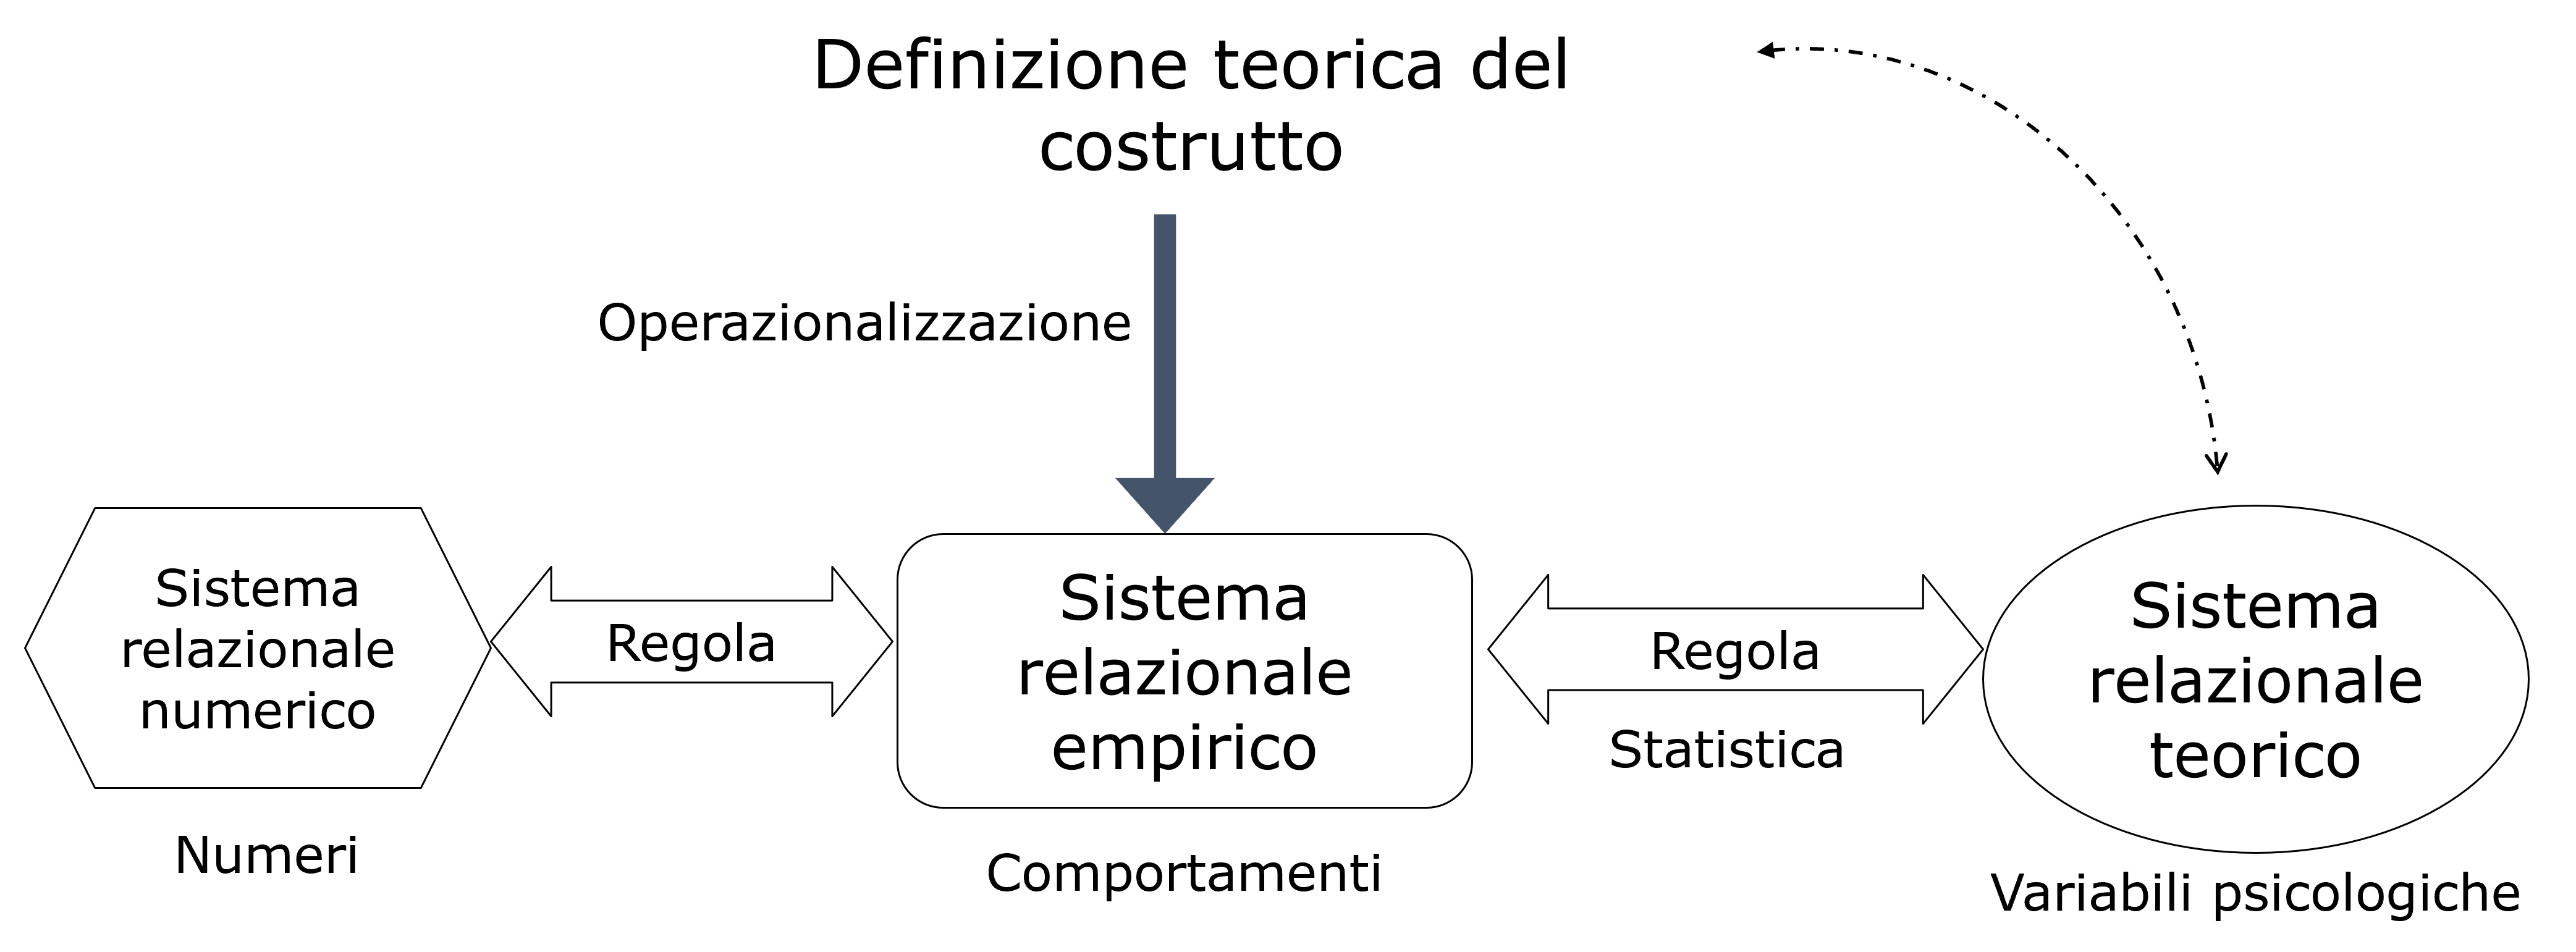
\includegraphics[width=.9\linewidth]{misura.png}
	\end{figure}
	
\vskip0pt plus 1filll

\color{template}\rule{0.30\linewidth}{0.5pt}\\
\color{black}
\scriptsize{Immagine adattata da Chiorri, C. (2023). \emph{Teoria e Tecnica Psicometrica, 2 ed.}, McGraw-Hill}

\end{frame}

\begin{frame}{Operazionalizzare}
	
	Si tratta della ``traduzione'' in comportamenti osservabili ed oggettivi di variabili latenti psicologiche \emph{non direttamente osservabili}
	
	La definizione teorica del costrutto diventa di vitale importanza per la definizione dei comportamenti osservabili ad esso legati... La misurazione del costrutto dipende proprio da questi!
	
	\begin{block}{Dominio di contenuto}
		
		Universo dei possibili comportamenti che, coerentemente con la definizione, possono rappresentare le operazionalizzazioni del costrutto 
		
		Quando è molto ampio $\rightarrow$ \emph{facets}
		
	\end{block}
\end{frame}

\begin{frame}{L'estroversione}
	\begin{spacing}\Factor
		\begin{table}
		\begin{tabular}{l l}
		\multicolumn{2}{c}{ESTROVERSIONE}\\
&  \\
		\hline
		Facets	&	Aggettivi prototipici	\\\hline
		Socievolezza	&	Socievole	\\
		Assertitivtà	&	Deciso	\\
		Attività	&	Energico	\\
		Ricerca di stimoli 	&	Avventuroso	\\
		Emozioni positive	&	Entusiastico	\\
		Espansività	&	Espansivo	\\\hline
		
	\end{tabular}
		\end{table}

	\end{spacing}

\end{frame}

\begin{frame}{Facets dell'estroversione}
	\begin{table}
			\begin{tabular}{l l l}
			\multicolumn{1}{c}{\textbf{Socievolezza}}	&	\multicolumn{1}{c}{\textbf{Espansività}}	&	\multicolumn{1}{c}{\textbf{Ricerca di stimoli}}	\\
			Socievole	&	Espansivo	&	Avventuroso	\\
			Spontaneo	&	Amichevole	&	Intrapredente	\\
			Simpatico	&	Schietto	&	Audace	\\
			Festaiolo	&	Sincero	&	Sfacciato	\\
			\emph{Chiuso}	&	Aperto	&	Coraggioso	\\
			\emph{Riservato}	&	Comunicativo	&	\emph{Fifone}	\\
			\multicolumn{1}{c}{\textbf{Assertività}}	&	\multicolumn{1}{c}{\textbf{Emozioni positive}}	&	\multicolumn{1}{c}{\textbf{Attività}}	\\
			Deciso	&	Entusiatsico	&	Energico	\\
			Determinato	&	Brioso	&	Dinamico	\\
			Sicuro di sé	&	Gioioso	&	Attivo	\\
			Fiducioso	&	Solare	&	Vigoroso	\\
			Risoluto	&	Spensierato	&	Rapido	\\
			\emph{Timido}	&	\emph{Preoccupato}	&	\emph{Letargico}	\\
			
			
		\end{tabular}
	\end{table}

\end{frame}

\section[Scale di misura]{Scale di misura}

\begin{frame}{Misura delle variabili}{Stevens (1946)}
	
	\small
	Si differenziano in base alla quantità di informazione che può essere ricavata
	
	\begin{itemize}
	\item \textbf{Nominale}: Distingue un insieme di dati in diverse categorie
	\begin{quote}
		Si sa solo che se si appartiene a una certa categoria si ha quella caratteristica e non un'altra
	\end{quote}
	\item \textbf{Ordinale}: Distingue un insieme di dati in diverse categorie che sono ordinabili a seconda della quantità di caratteristica posseduta 
	\begin{quote}
		Non si conosce la distanza tra le categorie
	\end{quote}
	\item \textbf{Intervalli equivalenti} Distingue un insieme di dati in diverse categorie ordinabili. La distanza tra le categorie è nota perché c'è un'unità di misura
	\begin{quote}
		Lo 0 è un valore puramente arbitrario
	\end{quote}
	\item \textbf{A rapporti equivalenti}: Come la scala ad intervalli...ma lo 0 indica assenza di caratteristica (non è arbitrario ma è assoluto) 
	\end{itemize}
\end{frame}

\subsection{Scala nominale}
\begin{frame}
Sconnessi (\textbf{scala nominale}): comune di residenza, genere, patologia clinica ecc. Vale solo l'equivalenza ($=$ o $\neq$)

\begin{center}
	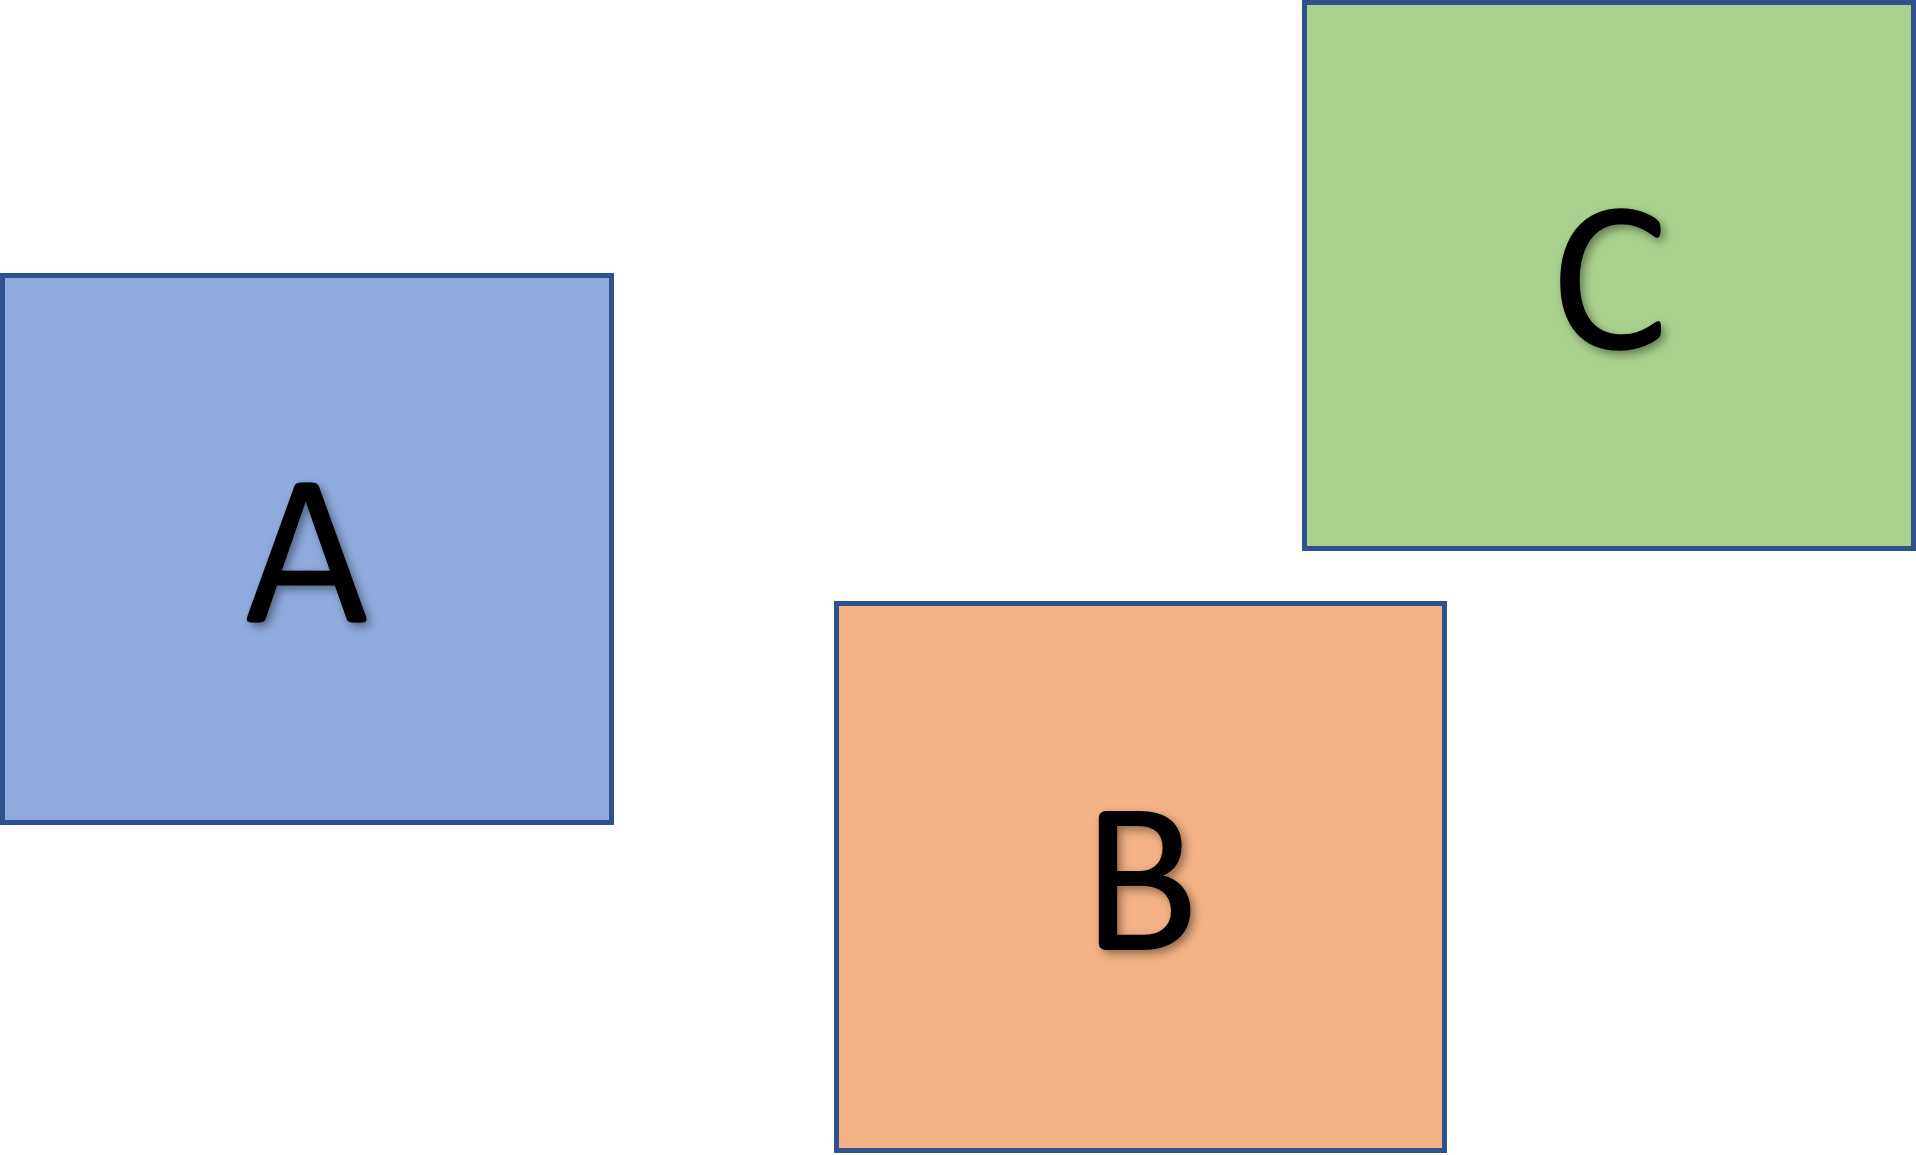
\includegraphics[width=.20\linewidth]{nominale.png}
\end{center}

Al posto di ``A'', ``B'', ``C'' si poteva scrivere $\alpha$, $\beta$ $\gamma$, 1,2,3 (ma i numeri valgono solo come etichette!)

Caratteristiche: 

\begin{itemize}
	\item  Categorie \textbf{distintive}: gli elementi che appartengono a categorie differenti vengono considerati di tipo diverso
	\item Categorie \textbf{mutualmente escludentesi}: ogni elemento può rientrare in una ed una sola categoria
	\item Categorie \textbf{Collettivamente esaustive}: tutti gli elementi vengono classificati nelle categorie della variabile, nessuno escluso
	
\end{itemize}
\end{frame}

\begin{frame}{Un esempio}
	\begin{figure}
		\centering
		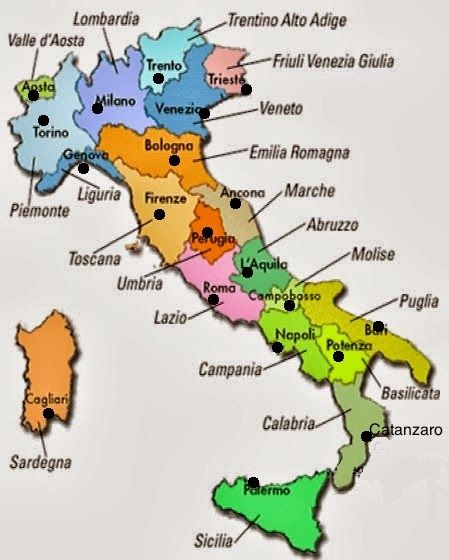
\includegraphics[width=0.4\linewidth]{regioni}
		\caption{Regione di nascita}
	\end{figure}
\end{frame}


\subsection{Scala ordinale}
\begin{frame}{Caratteri qualitativi ordinati}
	Modalità = attributi 
	
	Ordinati (\textbf{scala ordinale}): titolo di studio, gradimento di un prodotto, valutazione di una malattia (e.g., alto, medio, basso) ecc. Vale sia l'equivalenza ($=$ o $\neq$) sia l'ordinamento ($<$ o $>$)
	
	\begin{center}
		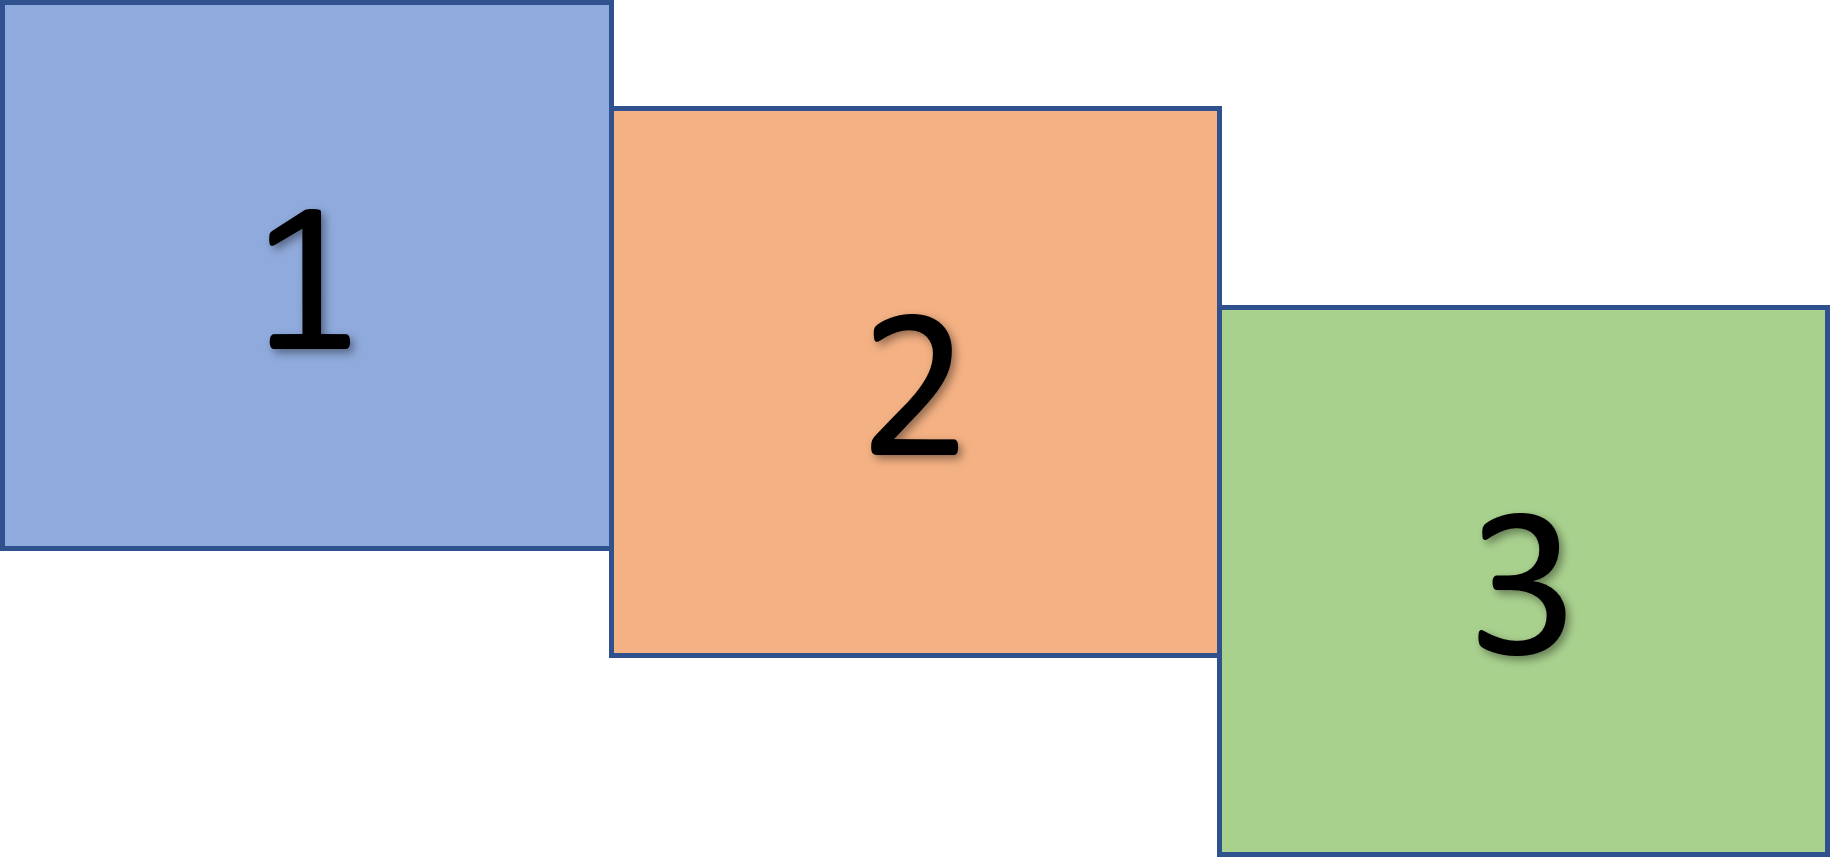
\includegraphics[width=.20\linewidth]{ordinale.png}
	\end{center}
	
	Le etichette numeriche valgono per il loro ordine (non ha senso compiere operazioni tra di loro)
\end{frame}

\begin{frame}{Un esempio}
	
	\begin{figure}
		\centering
		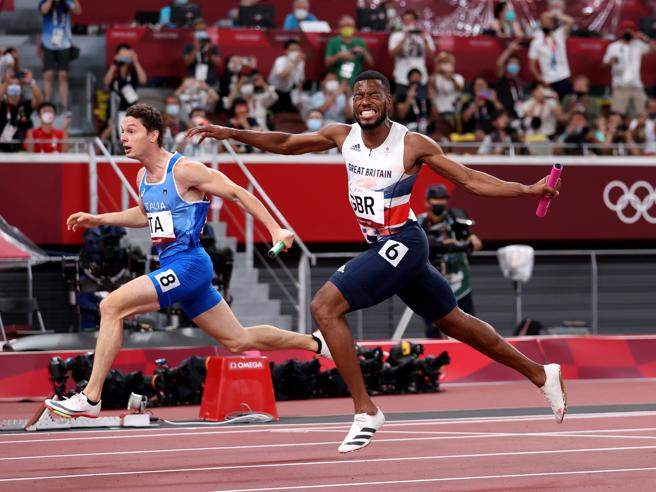
\includegraphics[width=0.5\linewidth]{ordinle}
		\caption{La staffetta 100$\times$4}
	\end{figure}
	
\end{frame}
\subsection{Scala a intervalli equivalenti}
\begin{frame}
	
	Lo $0$ è arbitrario, ma c'è un'\emph{unita di misura} per cui le categorie si trovano alla stessa distanza. Temperatura in Celsius, Q.I., scale di atteggiamento ecc. Vale equivalenza ($=$ o $\neq$), ordinamento ($<$ o $>$) e differenza ($+$ o $-$): 
	\begin{center}
		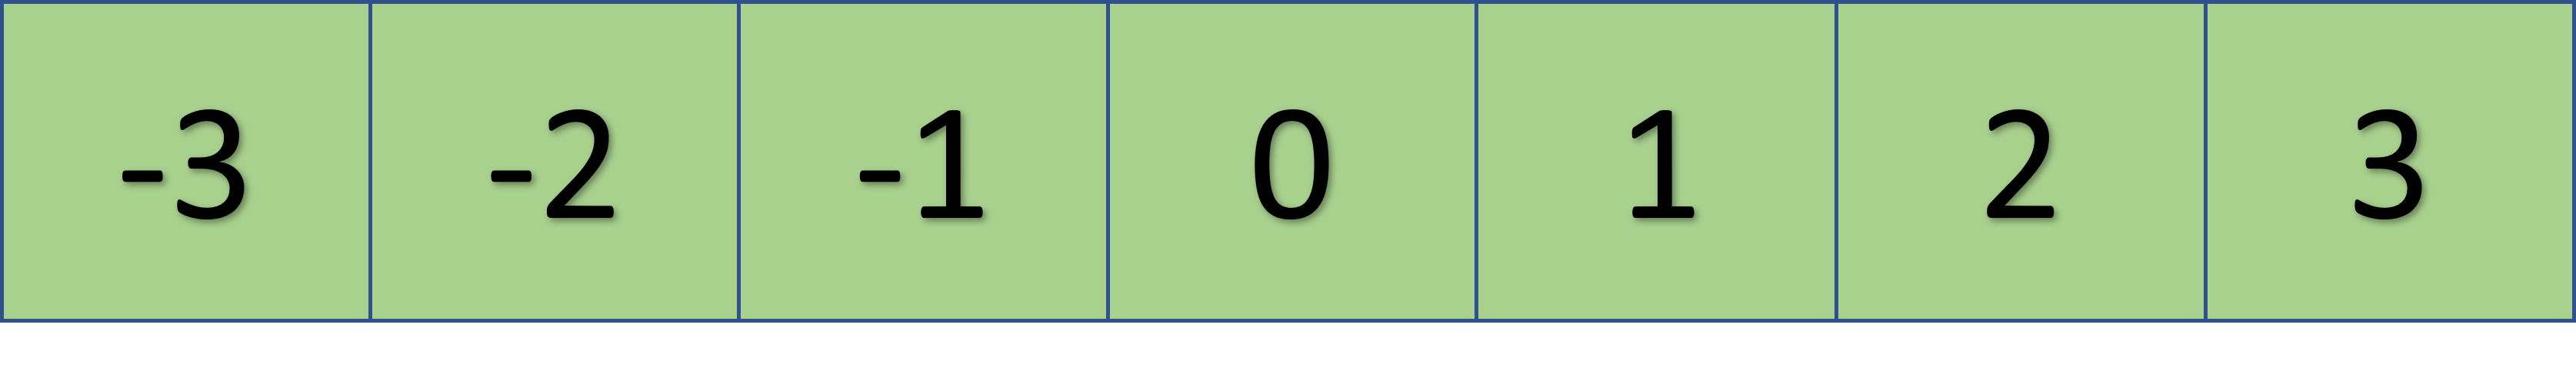
\includegraphics[width=0.5\linewidth]{intervalli.png}
	\end{center}
	
	\begin{figure}
		\centering
		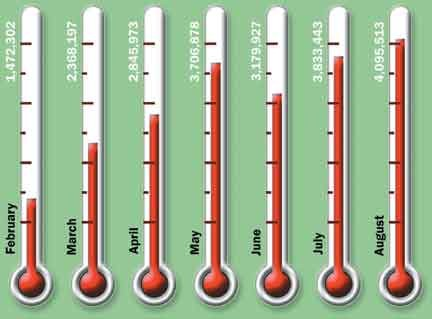
\includegraphics[width=0.8\linewidth]{termometroMulti.jpg}
	\end{figure}
	
\end{frame}

\begin{frame}
	\begin{columns}[T]
		\begin{column}{.50\linewidth}
		\begin{figure}
			\centering
			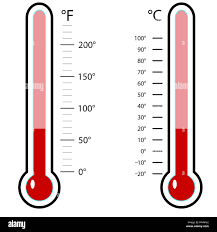
\includegraphics[width=\linewidth]{termometri}
		\end{figure}
		\end{column}
		
			\begin{column}{.50\linewidth}
Se ci sono 0°C, non vuol dire che non c'è calore! \\
Se ieri c'erano 5°C e oggi ce ne sono 10°C, possiamo dire che oggi fa più caldo di ieri e che ci sono 5°C più di ieri\\
Il fatto che lo 0 non sia arbitrario non ci permette di dire che oggi c'è il doppio del caldo di ieri! \\
Trasformando le due temperature in Fahrenheit si ottiene 41°F e 50°F... e la seconda non è più il doppio della prima!
		\end{column}
	\end{columns}

\end{frame}


\subsection{Scala a rapporti equivalenti}
\begin{frame}
	Lo 0 è assoluto, indica assenza del fenomeno. Peso, altezza, valori diagnostici. Vale equivalenza ($=$ o $\neq$),  ordinamento ($<$ o $>$), differenza ($+$ o $-$) e rapporto ($\times$ o $\div$)
	
	\begin{center}
		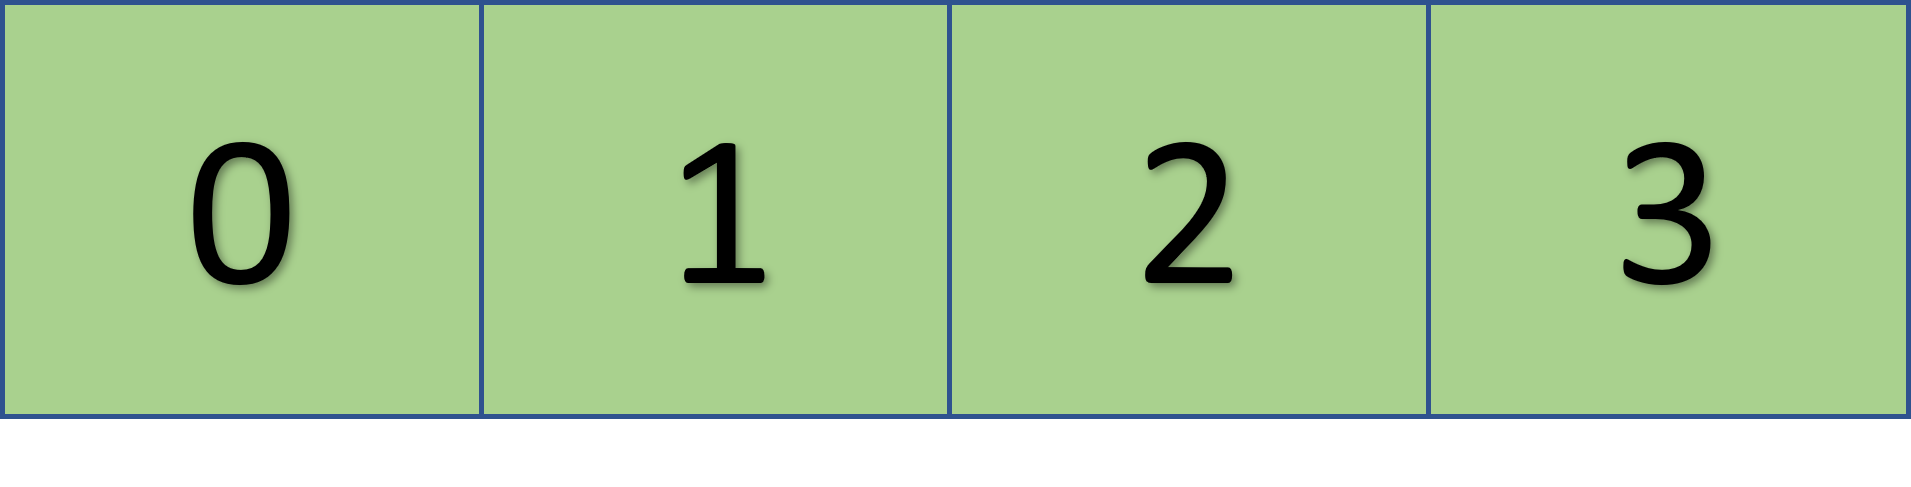
\includegraphics[width=0.40\linewidth]{rapporti.png}
	\end{center}
	
	
	% TODO: \usepackage{graphicx} required
	\begin{figure}
		\centering
		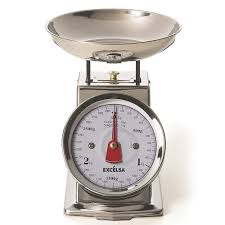
\includegraphics[width=0.4\linewidth]{bilancia}
	\end{figure}
	
\end{frame}

\begin{frame}
	% TODO: \usepackage{graphicx} required
	\begin{figure}
		\centering
		
\includegraphics[width=0.5\linewidth]{scale1}
	\end{figure}
\end{frame}

\section*{Riassunto}

\begin{frame}
	\begin{block}{Variabili qualitative}
		
		Nominali ed ordinali\\
		\textbf{Categorie}: Connotazioni/attributi assunte dalle variabili qualitative
	\end{block}
	
	\begin{block}{Variabili quantitative}
		
		A intervalli equivalenti e a rapporti equivalenti\\
		\textbf{Valori}: Connotazioni/misure assunte dalle variabili metriche che possono essere: 
		\begin{itemize}
		\item \textbf{Discreti}: insieme di modalità $\rightarrow$ insieme finito di soli numeri interi (e.g., numero di figli, numero di comportamenti patologici messi in atto in un lasso di tempo)
	
	\item \textbf{Continui}:  insieme di modalità $\rightarrow$ infinito, numeri reali (e.g., tempi di risposta a un esperimento)
		\end{itemize}
	\end{block}
\end{frame}


\section[Validità]{Validità e attendibilità delle misure}

\begin{frame}{Attendibilità}
	
	Grado in cui una procedura di misurazione produce lo stesso risultato in prove ripetute
	
	\begin{equation*}
		X = V + E
	\end{equation*}
	dove: \\
	$X$: misura rilevata\\
	$V$: parte vera\\
	$E$: errore: fluttuazioni casuali oppure costante e sistematico
	
	\pause
	L'attendibilità di una misura è la proporzione di $X$ che non riflette l'errore di misurazione: 
	\begin{equation*}
		\rho = \dfrac{V}{V + E}
	\end{equation*}
	
\end{frame}

\begin{frame}{Una nota sull'errore}
	\begin{block}{Errore casuale}
		
		Tutti quei fattori casuali che confondono la misurazione di qualunque fenomeno. \\
		Caratteristiche: 
		\begin{itemize}
			\item Ha media zero
		\item 	La correlazione fra punteggio vero ed errore è zero
			\item La correlazione fra errore e punteggio vero alla misurazione successiva è zero
			\item La correlazione fra errori di misurazioni diverse è zero
			
		\end{itemize}
		
	\end{block}
	
		\begin{block}{Errore sistematico (bias)}
		
		Effetto distorcente non casuale, sistematico
	\end{block}
\end{frame}

\begin{frame}

\begin{block}{Validità di costrutto}
	
	Quello che si sta misurando... è proprio quello che si voleva misurare e non altro!
	
	(Alcuni) Elementi utili per la \underline{validità di costrutto}:
	\begin{itemize}
		\item Chiara definizione del costrutto teorico
		\item Misurare il costrutto con metodi differenti
	\end{itemize} 
\end{block}	

\pause
\begin{block}{Validità statistica}
	
	Quello che stiamo iferendo a partire dalle analisi ha senso perché le analisi hanno senso! 
	
	(Alcuni) Elementi utili per la \underline{validità statistica}:
	\begin{itemize}
		\item Appropriatezza dei metodi statistici utilizzati sulla base delle variabili misurate
		\item Adeguatezza dell'ampiezza campionaria
	\end{itemize} 
	
\end{block}
\end{frame}

\begin{frame}
	\begin{block}{Validità esterna}
		
		Il grado in cui i risultati sono \emph{rappresentativi} della popolazione di interesse e il grado in cui sono \emph{replicabili}
		
			(Alcuni) Elementi utili per la \underline{validità esterna}:
		\begin{itemize}
			\item Il campione è rappresentativo della popolazione target
			\item La validità ecologica
		\end{itemize} 
	\end{block}
	
	\pause
		\begin{block}{Validità ecologica}
		
		Rappresenta la generalizzabilità dei risultati di una ricerca a quella che è la vita quotidiana 
		
		I dati raccolti devono essere rappresentativi del comportamento dell’individuo nella sua realtà abituale
		
	\end{block}
\end{frame}

\section[Misurazione esplicita]{Misurazione esplicita}

\begin{frame}{Item Vero/Falso}
	Sono item formulati in modo che l'unica possibile risposta possa essere Sì/No o Vero/Falso 
	
	\begin{quote}{Esempio}
		
		Mi commuovo quando vedo un film drammatico.
		\begin{itemize}
			\item Sì
			\item No
		\end{itemize}
	\end{quote}
	
	\begin{exampleblock}{Vantaggi}
		
		Sono estremamente facili da comprendere per chiunque 
	\end{exampleblock}
	
	\begin{alertblock}{Svantaggi}
		
		La scala di risposta potrebbe essere troppa riduttiva e particolarmente complessa per certe tipologie di persone
	\end{alertblock}
\end{frame}

\begin{frame}{Item a scelta multipla forzata}
	
	\begin{quote}
		
		Preferisco un lavoro nel quale: 
		
		\begin{enumerate}
			\item Posso crescere come persona
			\item Posso guadagnare bene
			\item Posso imparare cose nuove
		\end{enumerate}
	\end{quote}
	
		
	\vspace{2.5mm}
	Le opzioni di risposta sono realmente ordinabili? Sono anche solo comparabili?
	
	\pause
	\begin{exampleblock}{Narcissistic Personality Inventory}
		
		\pause
		\begin{enumerate}
			\item non sono né meglio né peggio di altre persone
			\item penso di essere una persona speciale 
		\end{enumerate}
		
		Una persona con un alto livello di narcisismo ha più probabilità di scegliere la seconda opzione
	\end{exampleblock}
\end{frame}

\begin{frame}{Rating scales}
	
	L'evoluzione delle scale con item Sì/No o Vero/Falso $\rightarrow$ aggiunta di livelli intermedi
	
	\emph{Summating rating scales:} Scale composte da diverse domande (\textbf{item}) il cui punteggio totale è ottenuto attraverso la somma dei punteggi alle valutazioni fornite ad ogni item
	
	\pause
	\begin{block}{Assunzione}
		
		Il costrutto latente si muove lungo un continuum sottostante alle opzioni di risposte, ovvero è possibile dare una quantità alla variabile psicologica misurata a seconda dell'opzione di risposta scelta. 
		\end{block}
		

\end{frame}

\begin{frame}

		
		Esprimere il proprio livello di accordo con l'affermazione ``Sono una persona organizzata'' secondo le seguenti opzioni di risposta: 
		
		\begin{center}
			Per niente d'accordo:	$\square$ \hspace{2mm} $\square$ \hspace{2mm} $\square$ \hspace{2mm} $\square$ \hspace{2mm} $\square$: Completamente d'accordo
		\end{center}

L'assunzione è che il livello di accordo con l'affermazione vari lungo un continuum e che questo continuum sia delimitato dagli ancoraggi ``Per niente d'accordo'' e ``Completamente d'accordo'': 

\pause
\begin{figure}
	\centering
	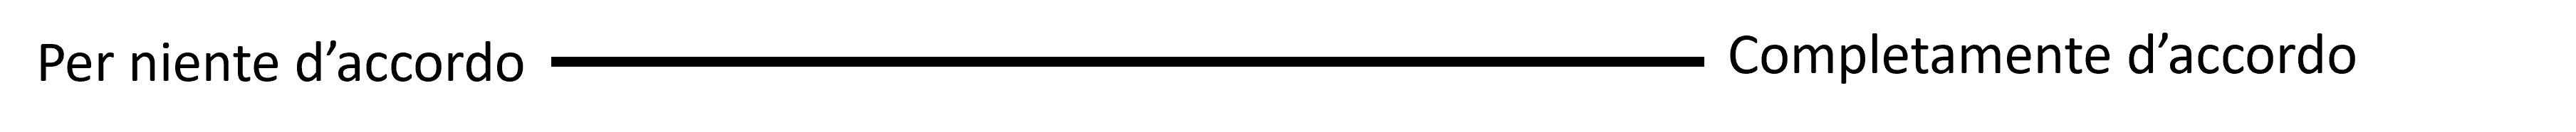
\includegraphics[width=0.9\linewidth]{accordo}
\end{figure}

\end{frame}

\begin{frame}{``Sono una persona organizzata''}{Indicare il grado di accordo con l'affermazione}
	
	\begin{block}{Barrare il valore numerico corrispondente}
		
		\begin{tabular}{p{2cm} p{2cm}  p{2cm}  p{2cm}  p{2cm} }
			Per niente & & & & Completamente \\
			1 & 2 & 3 & 4& 5 \\
		\end{tabular}
	\end{block}
	
		\begin{block}{Barrare la casella}
			
		\begin{tabular}{p{2cm} p{2cm}  p{2cm}  p{2cm}  p{2cm} }
			Per niente & & & & Completamente \\
			$\square$ & $\square$ & $\square$ & $\square$& $\square$ \\
		\end{tabular}
	\end{block}
	
\begin{block}{Segnare il numero}
	
	``Sono una persona organizzata'': \hspace{2cm} \large $\square$
\end{block}

	
\end{frame}

\begin{frame}{Visual Analougue Scale}

Molto utilizzate anche in psicologia dello sviluppo 

	\begin{figure}
		\centering
		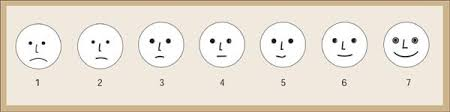
\includegraphics[width=0.7\linewidth]{vas}
	\end{figure}

\end{frame}

\begin{frame}{Domini}
	
	\begin{block}{Accordo}
		
		Indicare il grado di accordo con un'affermazione
		
		Ad esempio:\\
	\emph{Sono una persona organizzata} 
	\begin{center}
		Per niente d'accordo:	$\square$ \hspace{1.5mm} $\square$ \hspace{1.5mm} $\square$ \hspace{1.5mm} $\square$ \hspace{1.5mm} $\square$: Completamente d'accordo
	\end{center}
	\end{block}
	
		\begin{block}{Intensità}
		
	Dare una valutazione vera e propria rispetto a un argomento in termini di buono/cattivo, insufficiente/sufficiente, importante/non importante, eccetera. 
	
	Ad esempio: \\
	\emph{Indicare il proprio livello di competenze informatiche}
	\begin{center}
		5 $=$ alto; \hspace{1.5mm} 4 $=$ medio-alto; \hspace{1.5mm} 3 $=$ medio; \hspace{1.5mm} 2 $=$ medio-basso; \hspace{1.5mm} 1 $=$ basso
	\end{center}
	\end{block}
	

\end{frame}

\begin{frame}
	\small
		\begin{block}{Frequenza}
		
		Indicare la frequenza con cui vengono messi in atto i comportamenti o vengono sperimentati i vissuti descritti dall'item
		
		Ad esempio: \\
		\emph{Nell'ultimo anno, mi sono sentito ansioso:}
		\begin{center}
	Mai	$\square$ \hspace{1.5mm} Raramente $\square$ \hspace{1.5mm} Qualche volta $\square$ \hspace{1.5mm} Spesso $\square$ \hspace{1.5mm} Sempre $\square$
		\end{center}
	\end{block}
	
	\pause
	\begin{center}
		Attenzione!
	\end{center}
	
	Cosa vuole dire ``Spesso''? E ``Qualche volta''? Vogliono dire la stessa cosa per tutt*?
	
	\begin{columns}[T]
		\begin{column}{.50\linewidth}
			\begin{center}
				Bassa frequenza
			\end{center}
			\begin{enumerate}
				\item Mai 
				\item Circa una volta l'anno
				\item Circa due volte l'anno
				\item Due volte al mese 
				\item Più di due volte al mese
			\end{enumerate}
		\end{column}
		\begin{column}{.50\linewidth}
					\begin{center}
			Alta frequenza
		\end{center}
		\begin{enumerate}
			\item Due volte al mese o meno 
			\item Una volta a settimana
			\item Due volte a settimana
			\item Tutti i giorni 
			\item Diverse volte al giorno
		\end{enumerate}
		\end{column}
	\end{columns} 
\end{frame}

\begin{frame}{Quanti punti?}
	Come regola generale, più è alto il numero di punti della scala, maggiore è poi l'attendibilità della misura
	
	Solitamente si considerano scale con un numero di punti tra 4 e 7 $\rightarrow$ Più di 7 punti sono ``Inutili''
	
	Numero dispari o numero pari di punti? 
	
	Un numero dispari di punti permette l'alternativa neutra: 
	
	\begin{itemize}
		\item Ci sono dei casi (e.g., valutazione di soddisfazione per un servizio) dove ha senso avere un'alternativa neutra 
		\item In altri casi (e.g., valutazione degli atteggiamenti verso un gruppo sociale) l'alternativa neutra funge da ``rifugio'' per non sbilanciarsi
	\end{itemize}
\end{frame}


\begin{frame}{Criticità}
	\begin{block}{Acquiescienza}
		
		Essere sistematicamente d'accordo con le affermazioni proposte dagli item
	\end{block}
	
\begin{block}{Estremismo}
	
	Scegliere sempre le risposte estreme
\end{block}

\begin{block}{Evasività}
	
	Scegliere sempre i punti centrali della scala o le risposte ``Non so''
\end{block}

\begin{block}{Desiderabilità sociale}
	
Rispondere in modo da mostrarsi delle belle persone sempre e comunque	
\end{block}

\end{frame}
\section[Misurazione implicita]{Misurazione implicita: Definizioni ed evoluzione}

\begin{frame}
	\vskip0pt plus 1fill
	Secondo Greenwald \& Banaji (1995), gli atteggiamenti impliciti sono definiti come:
	
	\vspace{5mm}
	\begin{quote}
		Introspectively unidentified -- or inaccurately identified -- traces of past experience that mediate favorable or unfavorable feelings, thoughts, or actions toward social objects
	\end{quote}

\begin{center}
	\begin{large}
		IMPLICITO $=$ INCONSAPEVOLE
	\end{large}
\end{center}

Gli atteggiamenti impliciti si esprimono attraverso le cosiddette \textbf{associazioni automatiche}


\vskip0pt plus 1filll

\color{template}\rule{0.30\linewidth}{0.5pt}\\
\color{black}
\scriptsize{Greenwald, A. G., \& Banaji, M. R. (1995) Implicit Social Cognition: Attitudes, Self-Esteem, and Stereotypes.\emph{ Psychological Review}, 102-1, doi: 10.1037/0033-295X.102.1.4}


\end{frame}

\begin{frame}{Associazioni automatiche}
	\begin{center}
		
\includegraphics[width=.50\linewidth]{snakeFlower.png}
	\end{center}

\begin{itemize}
	\item Non controllabili
	\item Attivate da stimoli ``triggering'' 
	\item Non accessibili attraverso l'introspezione 
	\item Veloci e quasi immediati
\end{itemize}
	
	
\end{frame}

\begin{frame}{Associazioni automatiche e l'inconscio}
	Studiare le associazioni automatiche  $=$ Studiare gli atteggiamenti impliciti
	
	\vspace{3.5mm}
	\begin{center}
		
\includegraphics[width=.10\textheight]{down.png}
		
		\vspace{3.5mm}
		Avere accesso all'inconscio e poterlo (finalmente!) studiare con un approccio scientifico
	\end{center}

\pause

\centering

\includegraphics[width=.50\linewidth]{wrong.jpg}

\end{frame}

\begin{frame}
	\vskip0pt plus 1filll
	
	Fazio \& Olson (2003):
	
	\vspace{3mm}
	
	\begin{quote}
		Essere rapidi nell'associare i serpenti ad aggettivi o parole con valenza negativa non implica che non sia consapevoli dei propri atteggiamenti negativi verso i serpenti!
	\end{quote}

	\vspace{1.45mm}
	
	L'unica cosa di cui si è realmente inconsapevoli è che qualcuno sta misurando gli atteggiamenti!
	
	L'atteggiamento (l'oggetto della misura) non è implicito, lo è il processo stesso di misurazione


	\vspace{1.5mm}
	Costrutti misurati implicitamente Vs. Costrutti inconsapevoli 

\vskip0pt plus 1filll

\color{template}\rule{0.30\linewidth}{0.5pt}\\
\color{black}
\scriptsize{Fazio, R. H., \& Olson, M. A. (2003). Implicit measures in social cognition research: Their meaning
	and use. \emph{Annual Review of Psychology, 54}(1), 297–
	327. https://doi.org/10.1146/annurev.psych.54.101
	601.145225}

\end{frame}

\subsection*{Implicit $=$ indirect}


\begin{frame}
	
	\begin{center}
		Da
		
		\vspace{3.5mm}
		Esplicito = consapevole Vs. Implicito = inconsapevole/Inconscio  
		
		\emph{Riferendosi alla natura dei costrutti}
		\vspace{3.5mm}
		
		a:
		
		\vspace{3.5mm}
		Esplicito = diretto Vs. Implicito = indiretto 
		
		\emph{Riferendosi alla natura della misurazione}
	\end{center}
	
	\vspace{3.5mm}
	Significato \emph{empirico} del termine implicito
\end{frame}

\begin{frame}
	\vskip0pt plus 1filll
	Banaji \& Greenwald (2013): 
	
	\vspace{5mm}
	\begin{quote}
		Definizione \underline{\textbf{teorica}} del termine implicito come inconscio e inconsapevole
	\end{quote}

\vspace{5mm}
Greenwald \& Banaji (2017), Greenwald \& Lai (2020): 

\vspace{5mm}
\begin{quote}
	
	Definizione \underline{\textbf{empirica}} del termine implicito come indiretto 

\end{quote}
\vskip0pt plus 1filll

\color{template}\rule{0.30\linewidth}{0.5pt}\\
\color{black}
\scriptsize{Banaji, M. R., \& Greenwald, A. G. (2013). \emph{Blindspot:
	Hidden biases of good people}. Delacorte Press,\\ 
Greenwald, A. G., \& Banaji, M. R. (2017). The
implicit revolution: Reconceiving the relation
between conscious and unconscious. \emph{American Psychologist, 72}(9), 861–871. https://doi.org/10.1037/
amp0000238\\
Greenwald, A. G., \& Lai, C. K. (2020). Implicit social
cognition. \emph{Annual Review of Psychology, 71}, 419–
445. https://doi.org/10.1146/annurev-psych-010419-
050837
}
\end{frame}

\begin{frame}{Perché...?}
	\begin{itemize}
		\item Mancanza di evidenza empirica scientifica per poter sostenere l'accesso all'inconscio 
		\item Problemi relativi alla validità di costrutto $\rightarrow$ cosa stiamo misurando? Siamo \emph{sicuri} di star misurando quello che pensiamo di misurare?  
		\item Definizione senza una teoria dietro 
	\end{itemize}
\end{frame}

\section[IAT]{Implicit Association Test}

\begin{frame}{Implicit Association Test}

	\tikzoverlay (n1) at (8cm, 0.5cm){%
		\begin{minipage}{0.3\linewidth}
			\centering	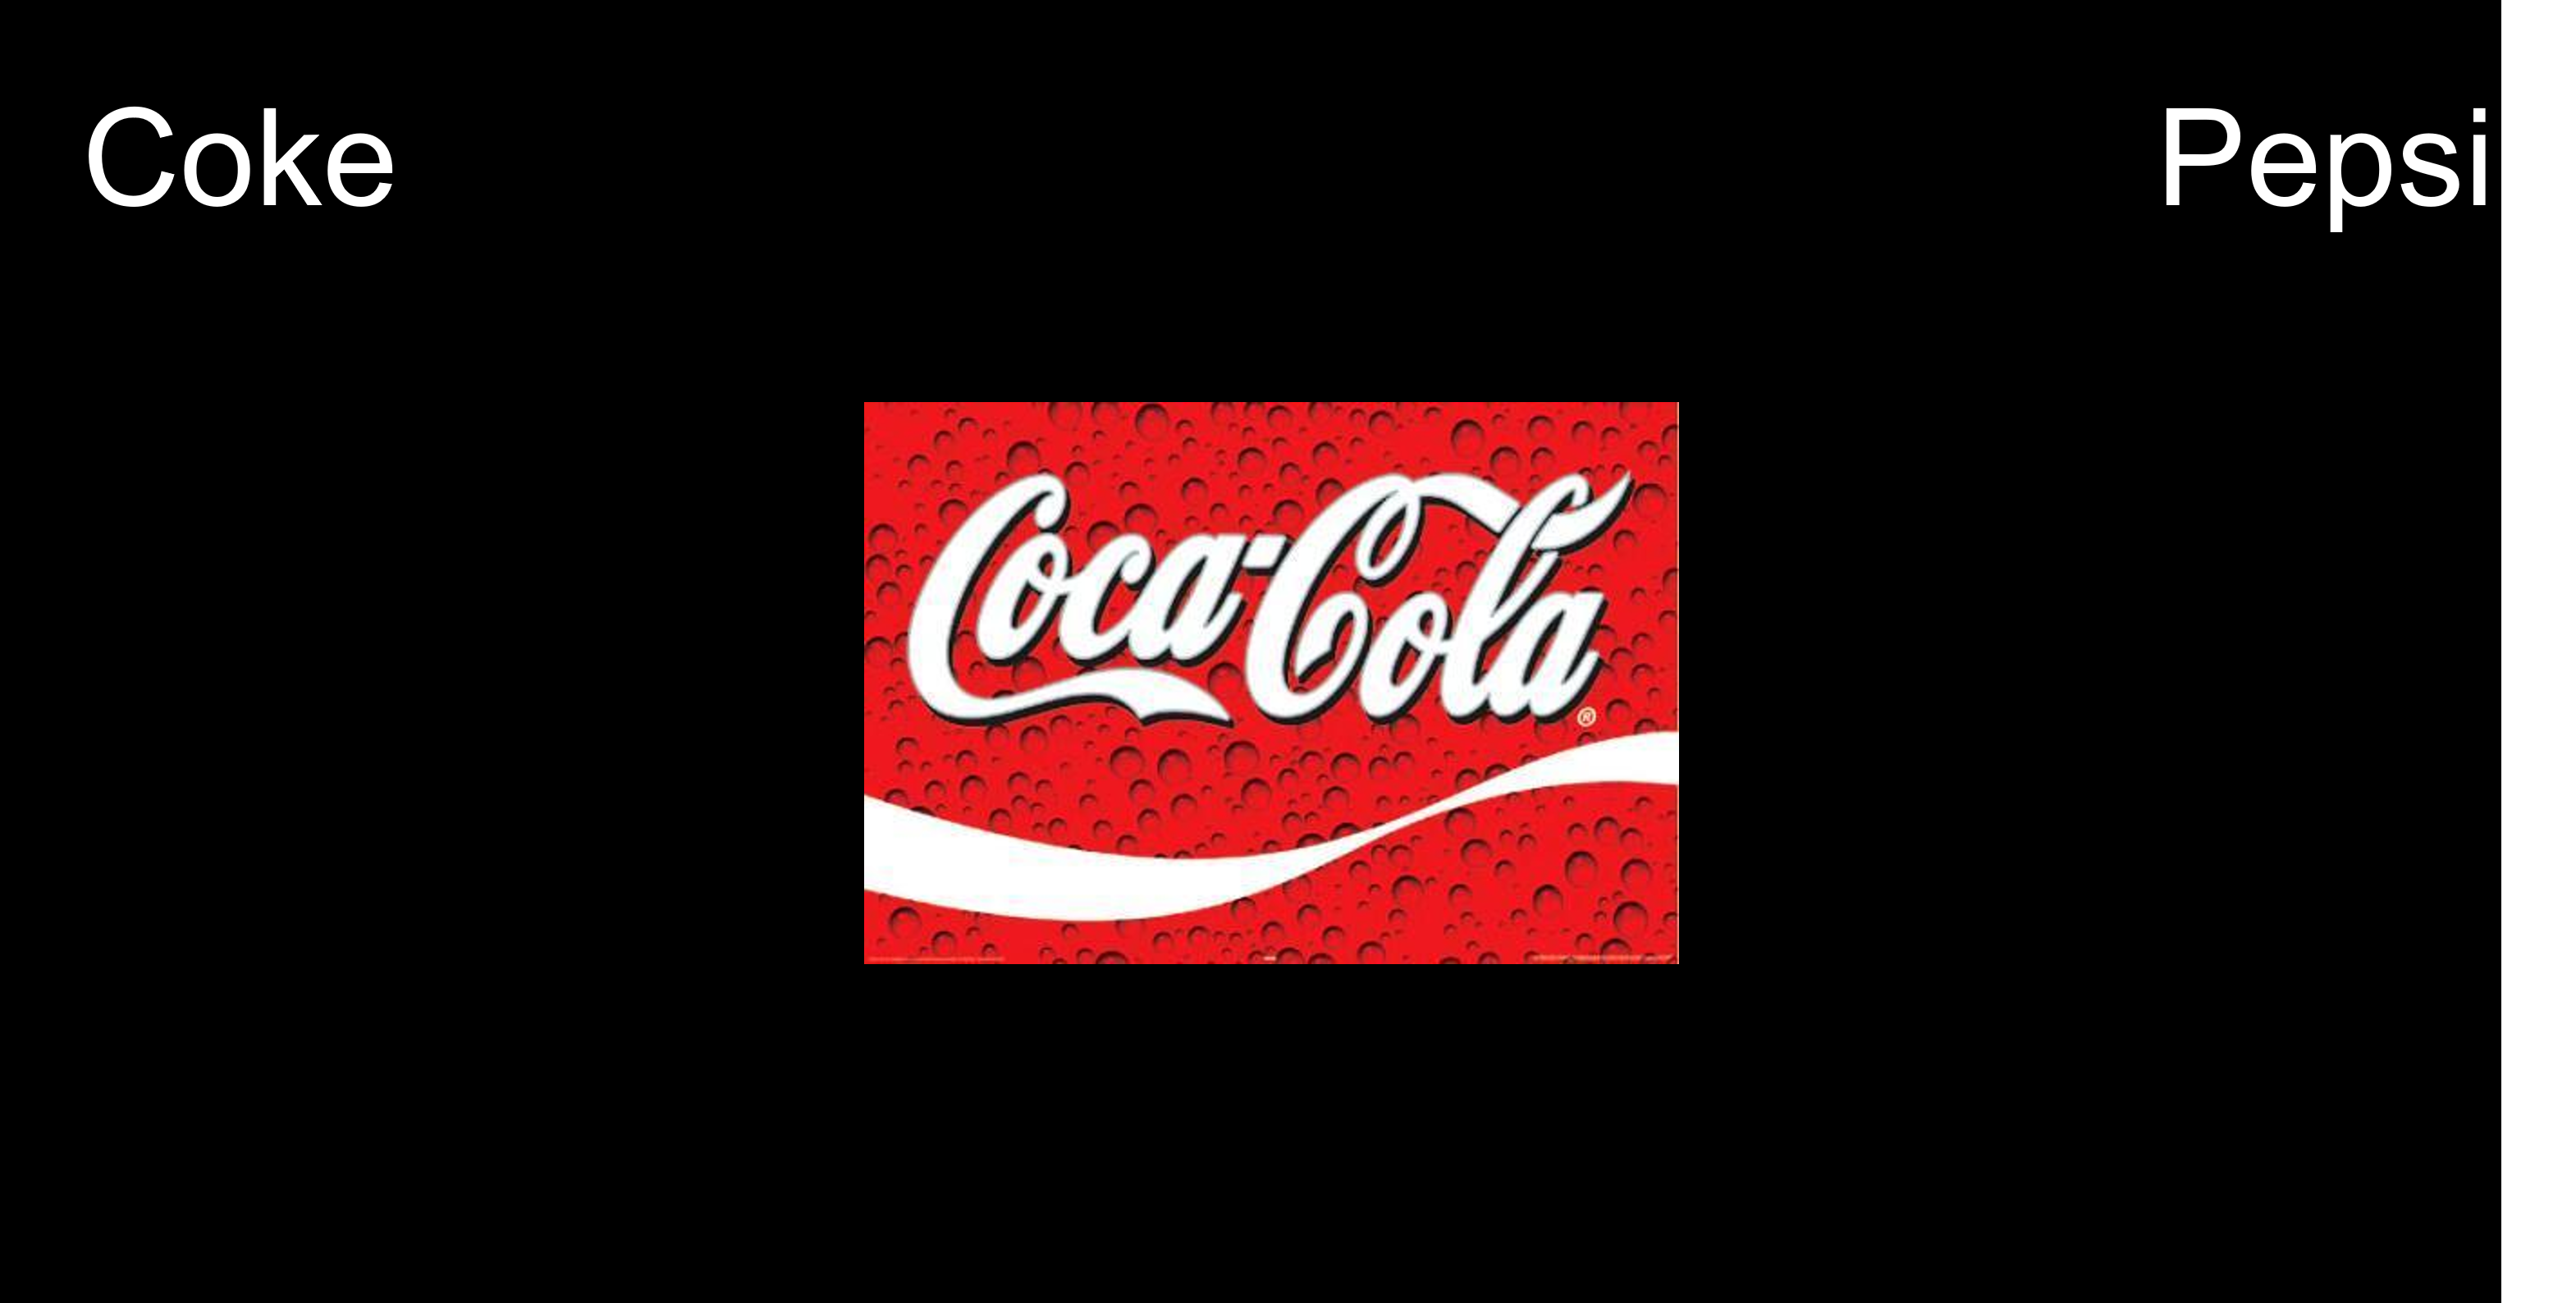
\includegraphics[width=\linewidth]{iatbase.png}
		\end{minipage}
	}; %

	Greenwald et al. (1998):
	
			\begin{table}
				\centering
				\caption{IAT}
				\begin{tabular}{c c c c }
					\hline
					Blocco	&	\# Trial	&	Tasto sinistro (E)	&	Tasto destro (I)	\\ \hline
					1	&	20	&	Good	&	Bad	\\
					2	&	20	&	Coke	&	Pepsi	\\
					\textcolor<2->{unipd}{3}	&	\textcolor<2->{unipd}{20}	&	\textcolor<2->{unipd}{Coke + Good}	&	\textcolor<2->{unipd}{Pepsi + Bad}	\\
					\textcolor<2->{unipd}{4}	&	\textcolor<2->{unipd}{40}	&	\textcolor<2->{unipd}{Coke + Good}	&	\textcolor<2->{unipd}{Pepsi + Bad}	\\
					5	&	20	&	Pepsi	&	Coke	\\
					\textcolor<3->{blu}{6}	&	\textcolor<3->{blu}{20}	&	\textcolor<3->{blu}{Pepsi + Good}	&	\textcolor<3->{blu}{Coke + Bad}	\\
					\textcolor<3->{blu}{7}	&	\textcolor<3->{blu}{40}	&	\textcolor<3->{blu}{Pepsi + Good}	&	\textcolor<3->{blu}{Coke + Bad}	\\
					\hline
				\end{tabular}
			\end{table}

	


	\vspace{2mm}
\begin{columns}
	\begin{column}{.50\linewidth}
	\onslide<2-> \textcolor{unipd}{Condizione Coke-Good/Pepsi-Bad}	
	\end{column}
\begin{column}{.50\linewidth}
	\onslide<3-> \textcolor{blu}{Condizione Pepsi-Bad/Coke-Good}	
\end{column}

\end{columns}




%\color{template}\rule{0.30\linewidth}{0.5pt}\\
%\color{black}
%Greenwald, A. G., McGhee, D. E., \& Schwartz,
%	J. L. K. (1998). Measuring individual differences
%	in implicit cognition: The implicit association test.
%	Journal of Personality and Social Psychology,
%	74(6), 1464–1480. https://doi.org/10.1037/0022-
%	3514.74.6.1464
\end{frame}


\begin{frame}
	\begin{columns}
		\column{.5\linewidth}
		\centering{\textcolor{unipd}{Coke-Good/Pepsi-Bad (CGPB)}}
		\begin{figure}
			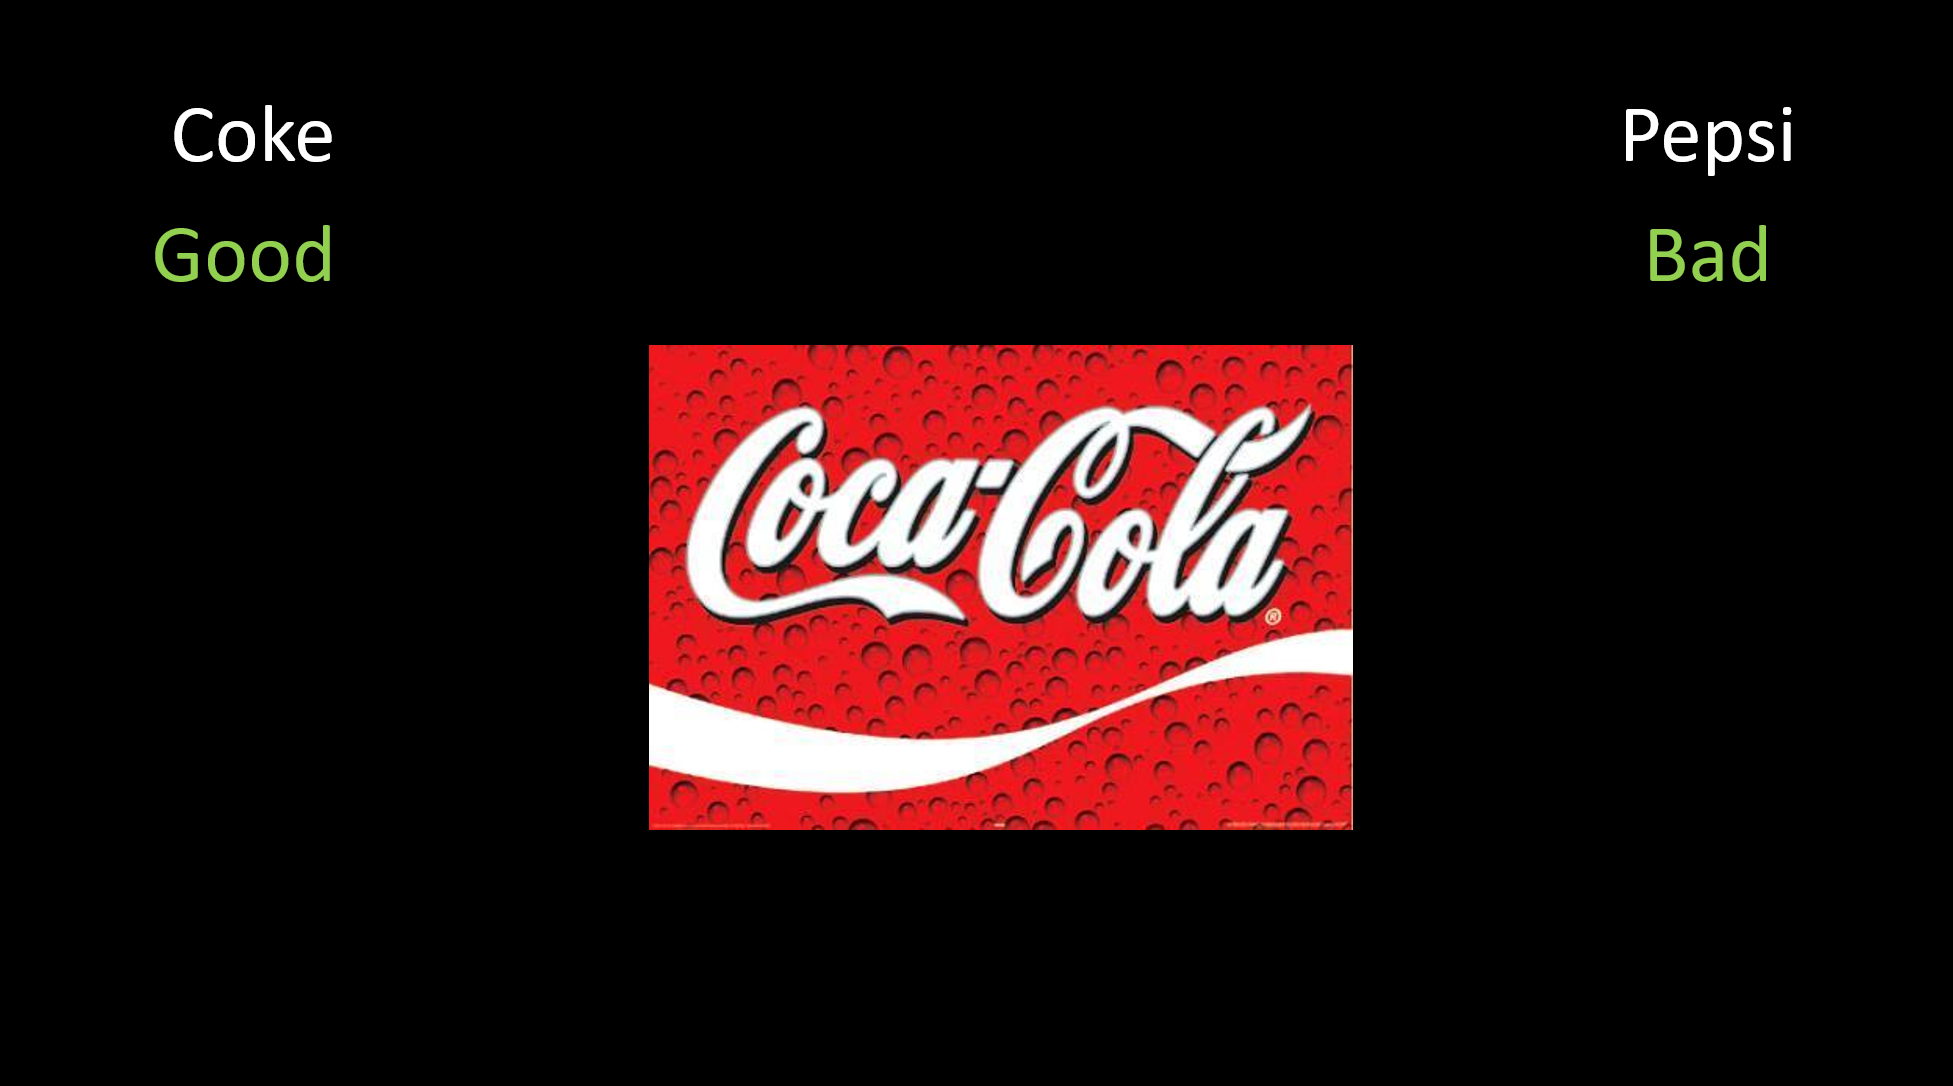
\includegraphics[width=\linewidth]{cocagood.png}
		\end{figure}
		
		\column{.5\linewidth}
		\centering{\textcolor{blu}{Pepsi-Good/Coke-Bad (PGCB)}}
		\begin{figure}
			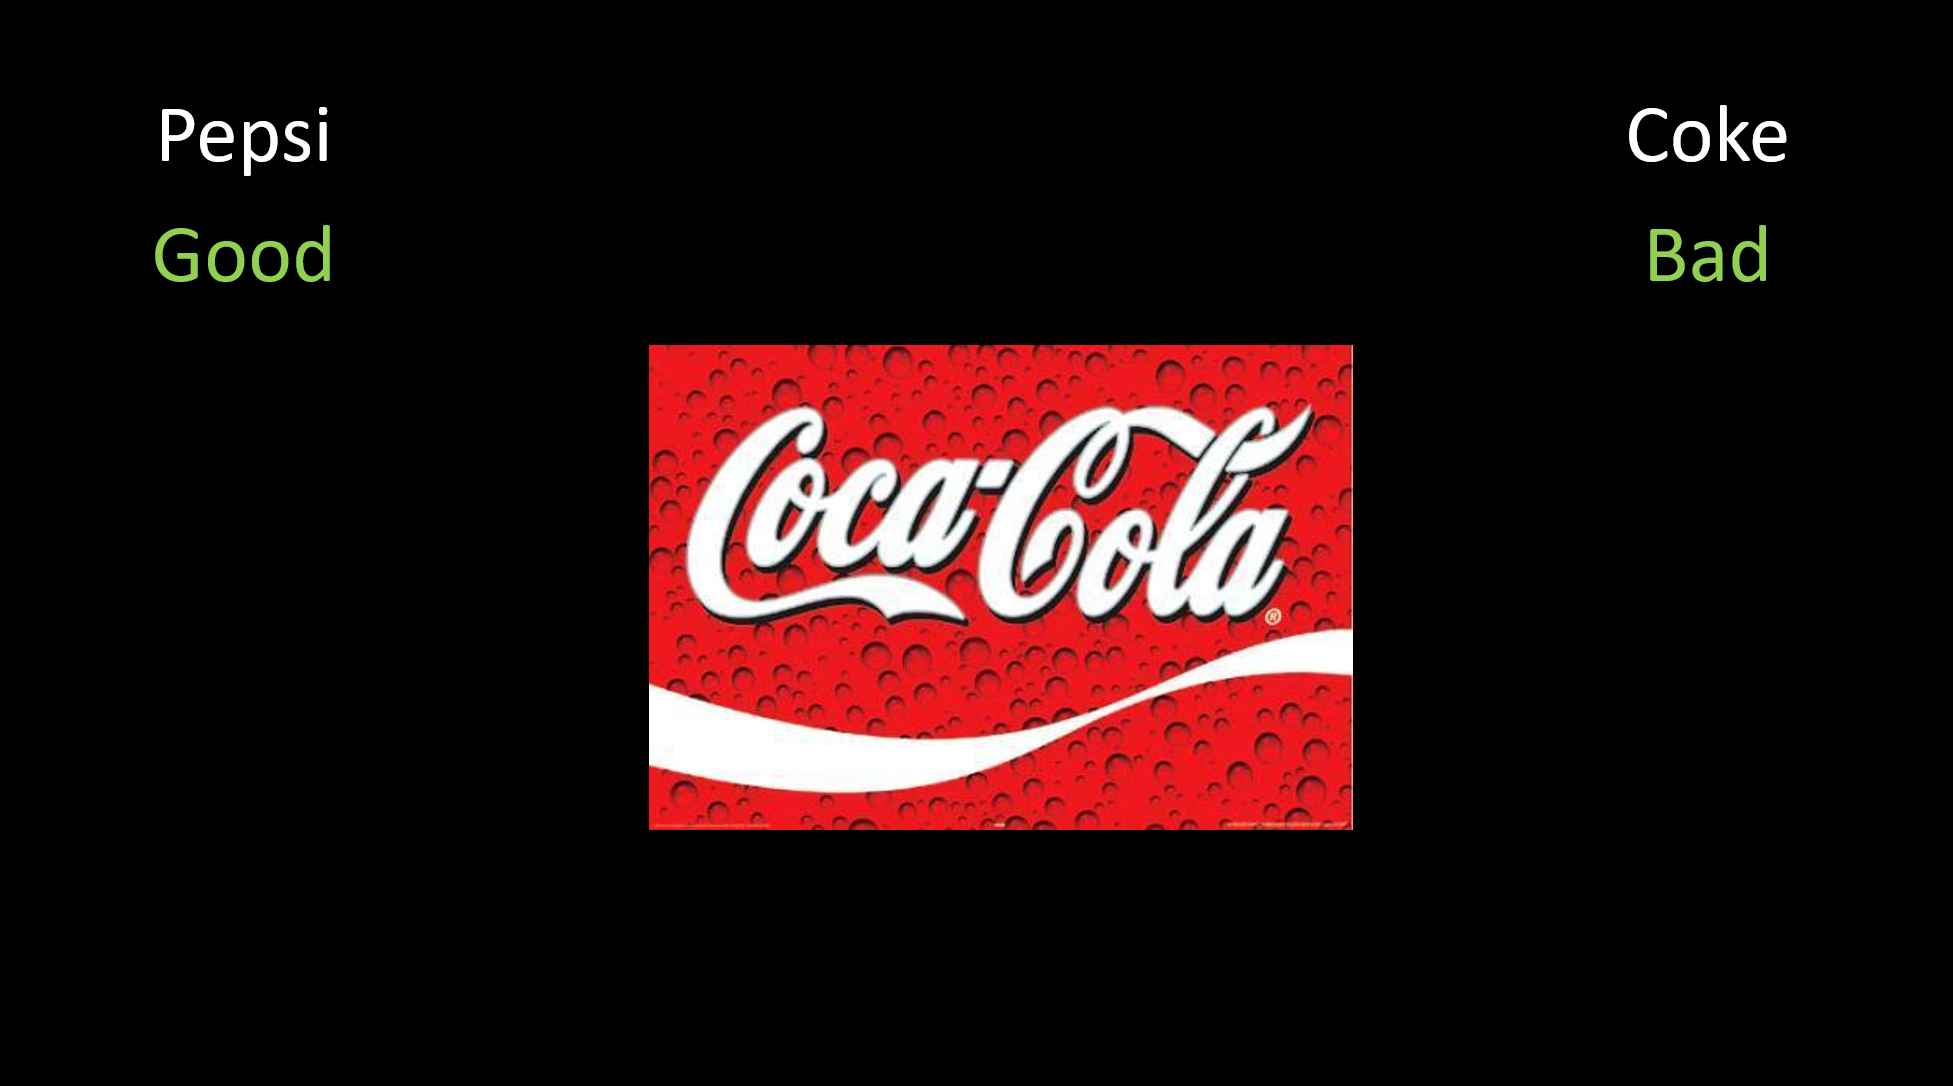
\includegraphics[width=\linewidth]{cocabad.png}
		\end{figure}
	\end{columns}

\end{frame}


\begin{frame}
	\begin{textblock*}{10cm}(0.5cm,1cm)
		{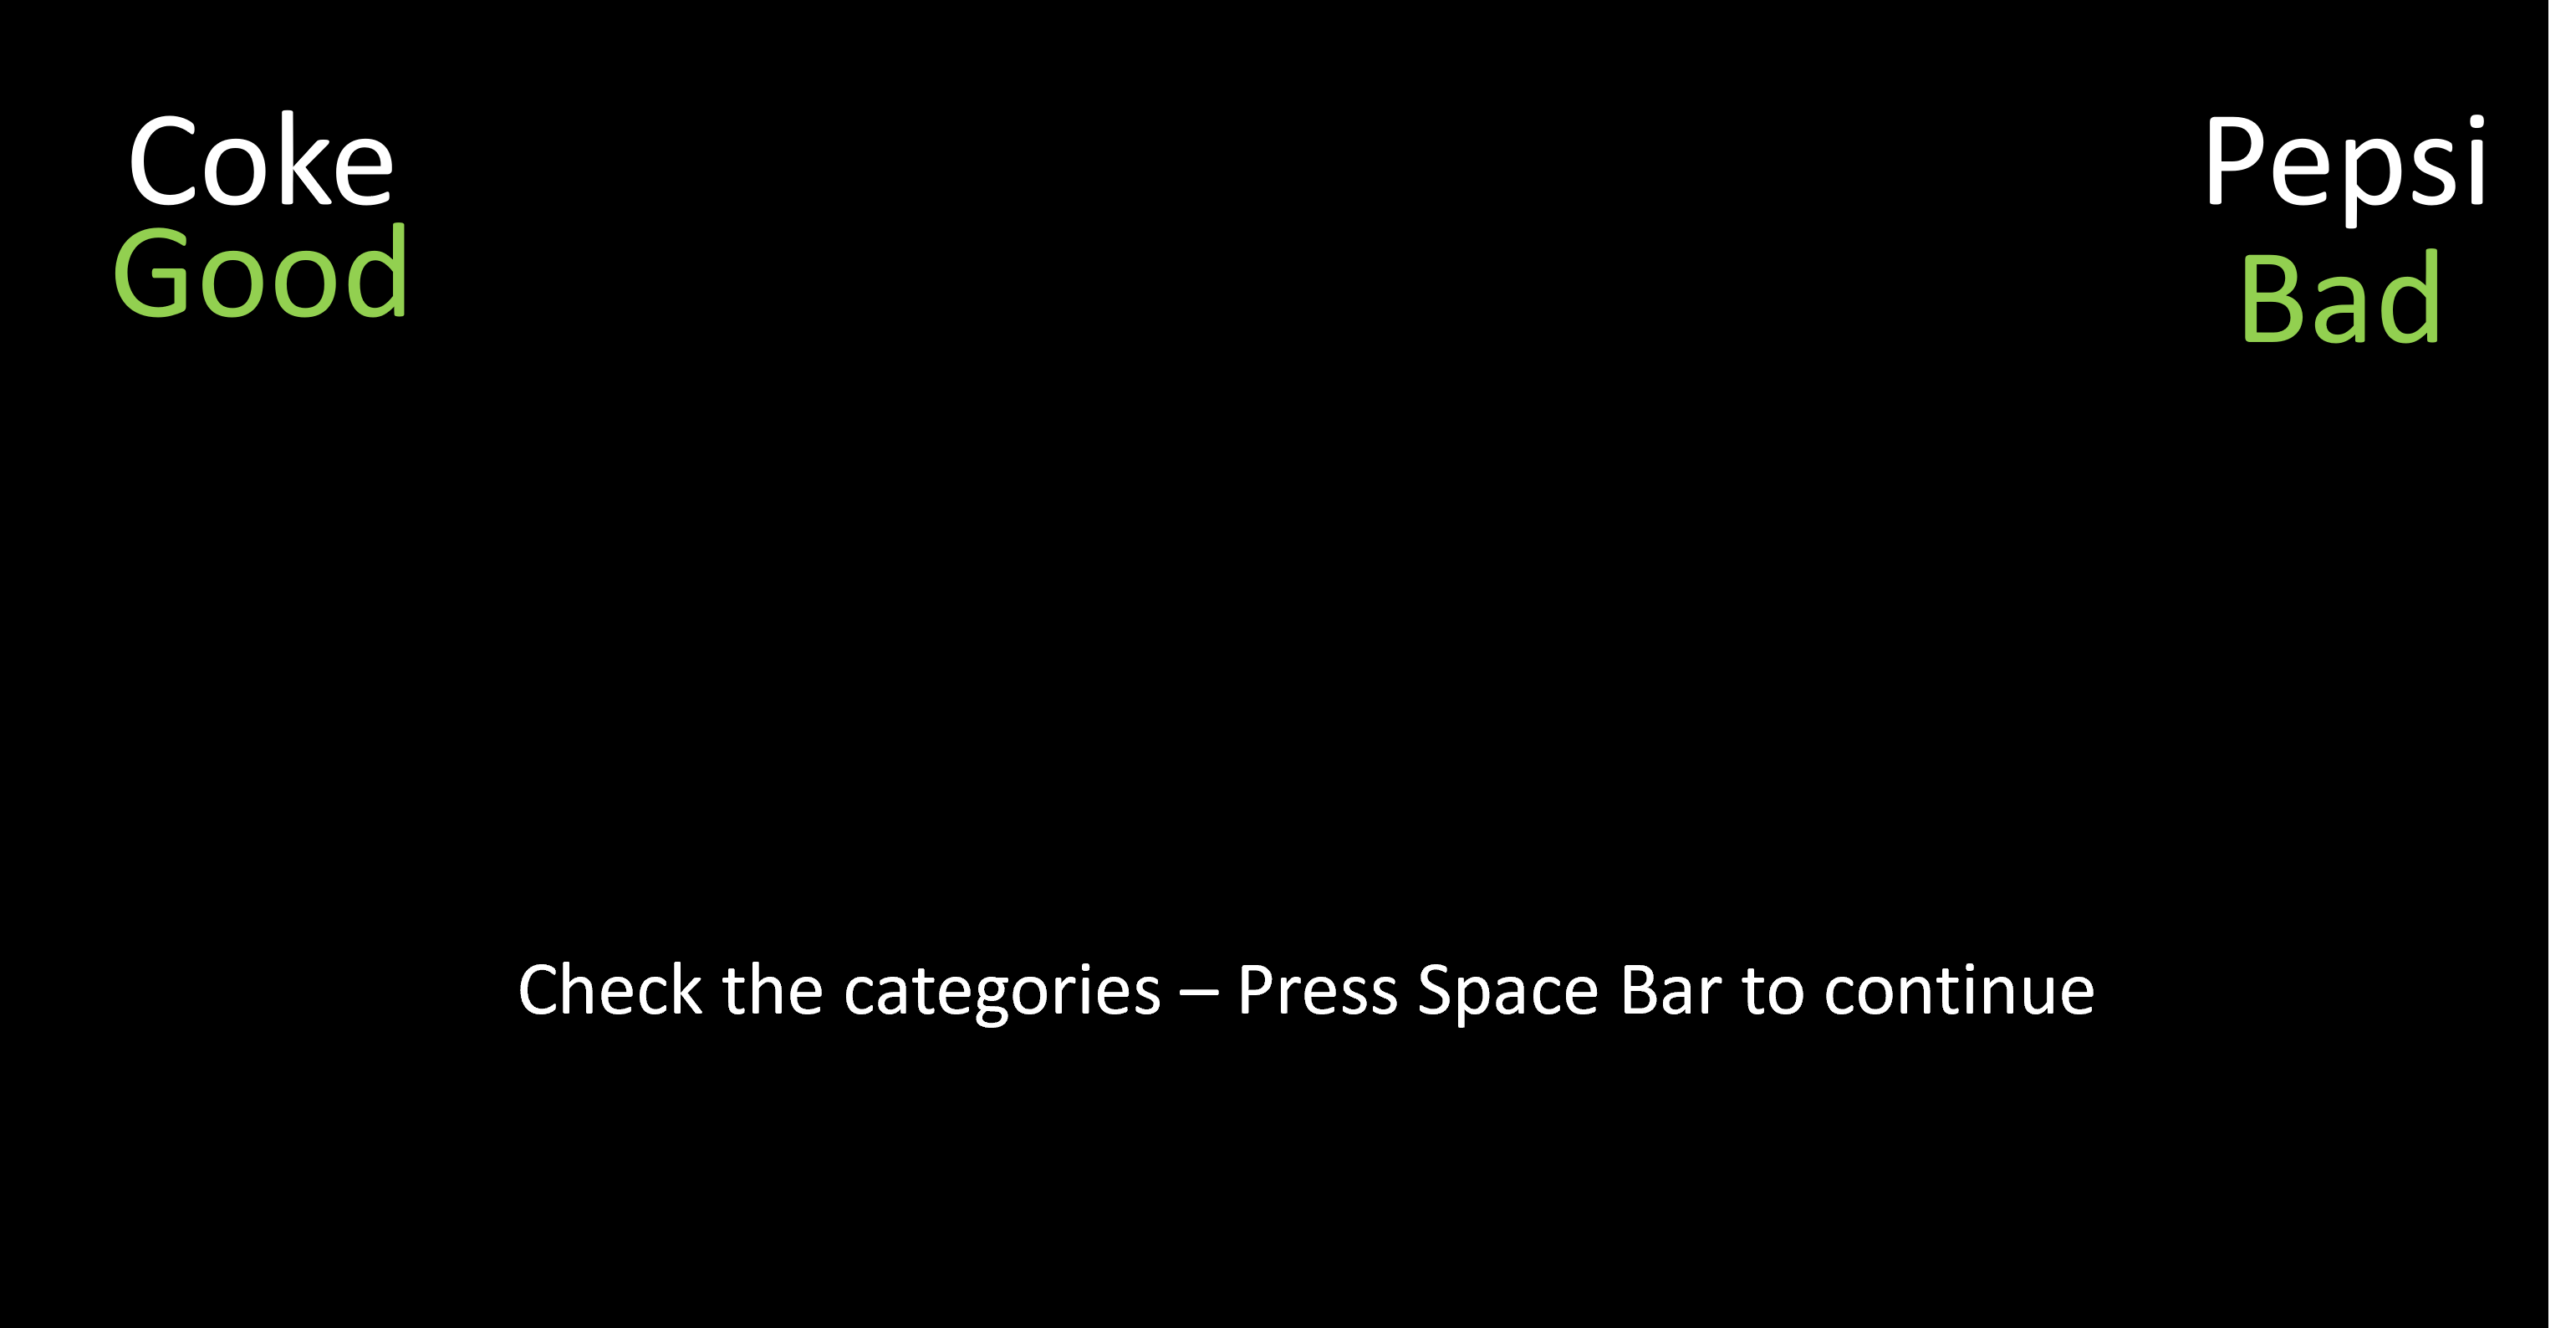
\includegraphics[width=\linewidth]{cokeIAT1.png}}
	\end{textblock*}
	\begin{textblock*}{10cm}(0.7cm,1.4cm)
		{\includegraphics<2->[width=\linewidth]{cokeIAT2.png}}
	\end{textblock*}
	\begin{textblock*}{10cm}(0.9cm,1.8cm)
		{\includegraphics<3->[width=\linewidth]{cokeIAT3.png}}
	\end{textblock*}
	\begin{textblock*}{10cm}(1.1cm,2.2cm)
		{\includegraphics<4->[width=\linewidth]{cokeIAT4.png}}
	\end{textblock*}
	\begin{textblock*}{10cm}(1.3cm,2.6cm)
		{\includegraphics<5->[width=\linewidth]{cokeIAT5.png}}
	\end{textblock*}
	
	\vskip0pt plus 1filll
	
	\onslide<2-2> Tasto E
	\onslide<3-3> Tasto I
	\onslide<4-4> Tasto E
	\onslide<5-5> Tasto I
	
\end{frame}

\subsection*{Scoring}

\begin{frame}{\emph{D} score}
	\vskip0pt plus 1filll
Greenwald et al. (2003)
	
	\vspace{5mm}
	\begin{columns}
		\begin{column}{.50\linewidth}
			$$D_{\mathrm{B6,B3}} = \frac{M_{\mathrm{B6}} - M_{\mathrm{B4}}}{sd_{\mathrm{B6, B3}}}$$
		\end{column}
		\begin{column}{.50\linewidth}
			$$D_{\mathrm{B7,B4}} = \frac{M_{\mathrm{B7}} - M_{\mathrm{B4}}}{sd_{\mathrm{B7, B4}}}$$
	\end{column}
	\end{columns}
	
	\vspace{5mm}
		\begin{equation*}
		D = \frac{D_{\mathrm{B6,B3}} + D_{\mathrm{B7,B4}}}{2}
	\end{equation*}
	
	\pause
	\vspace{5mm}
	Risposte errate? Risposte troppo veloci?
	
	\vskip0pt plus 1filll
	
	\color{template}\rule{0.30\linewidth}{0.5pt}\\
	\color{black}
	\scriptsize{Greenwald, A. G., Nosek, B. A., \& Banaji, M. R.
		(2003). Understanding and using the implicit association test: I. An improved scoring algorithm. \emph{Journal
		of Personality and Social Psychology, 85}(2), 197–
		216. https://doi.org/10.1037/0022-3514.85.2.197}
\end{frame}

\begin{frame}
	
	\begin{spacing}\Factor
		\begin{table}[th!]
			\centering
			\caption{\label{tab:overview} Panoramica degli algoritmi di scoring}
			\begin{tabularx}{\linewidth}{llll}
				\hline
				\emph{D score} & Risposte errate & Risposte troppo veloci\\\hline
				\emph{D1} & Built-in correction & No \\
				\emph{D2} & Built-in correction & Eliminare trials $<$ 400 \emph{ms} \\
				\emph{D3} & Mean (correct responses) + 2\emph{sd} & No\\
				\emph{D4} & Mean (correct responses) + 600 \emph{ms} & No \\
				\emph{D5} & Mean (correct responses) + 2\emph{sd} & Eliminare trials $<$ 400 \emph{ms}\\
				\emph{D6} & Mean (correct responses) + 600 \emph{ms} & Eliminare trials $<$ 400 \emph{ms} \\\hline
			\end{tabularx}
		\end{table}
	\end{spacing}
\end{frame}


\begin{frame}
	\begin{figure}
		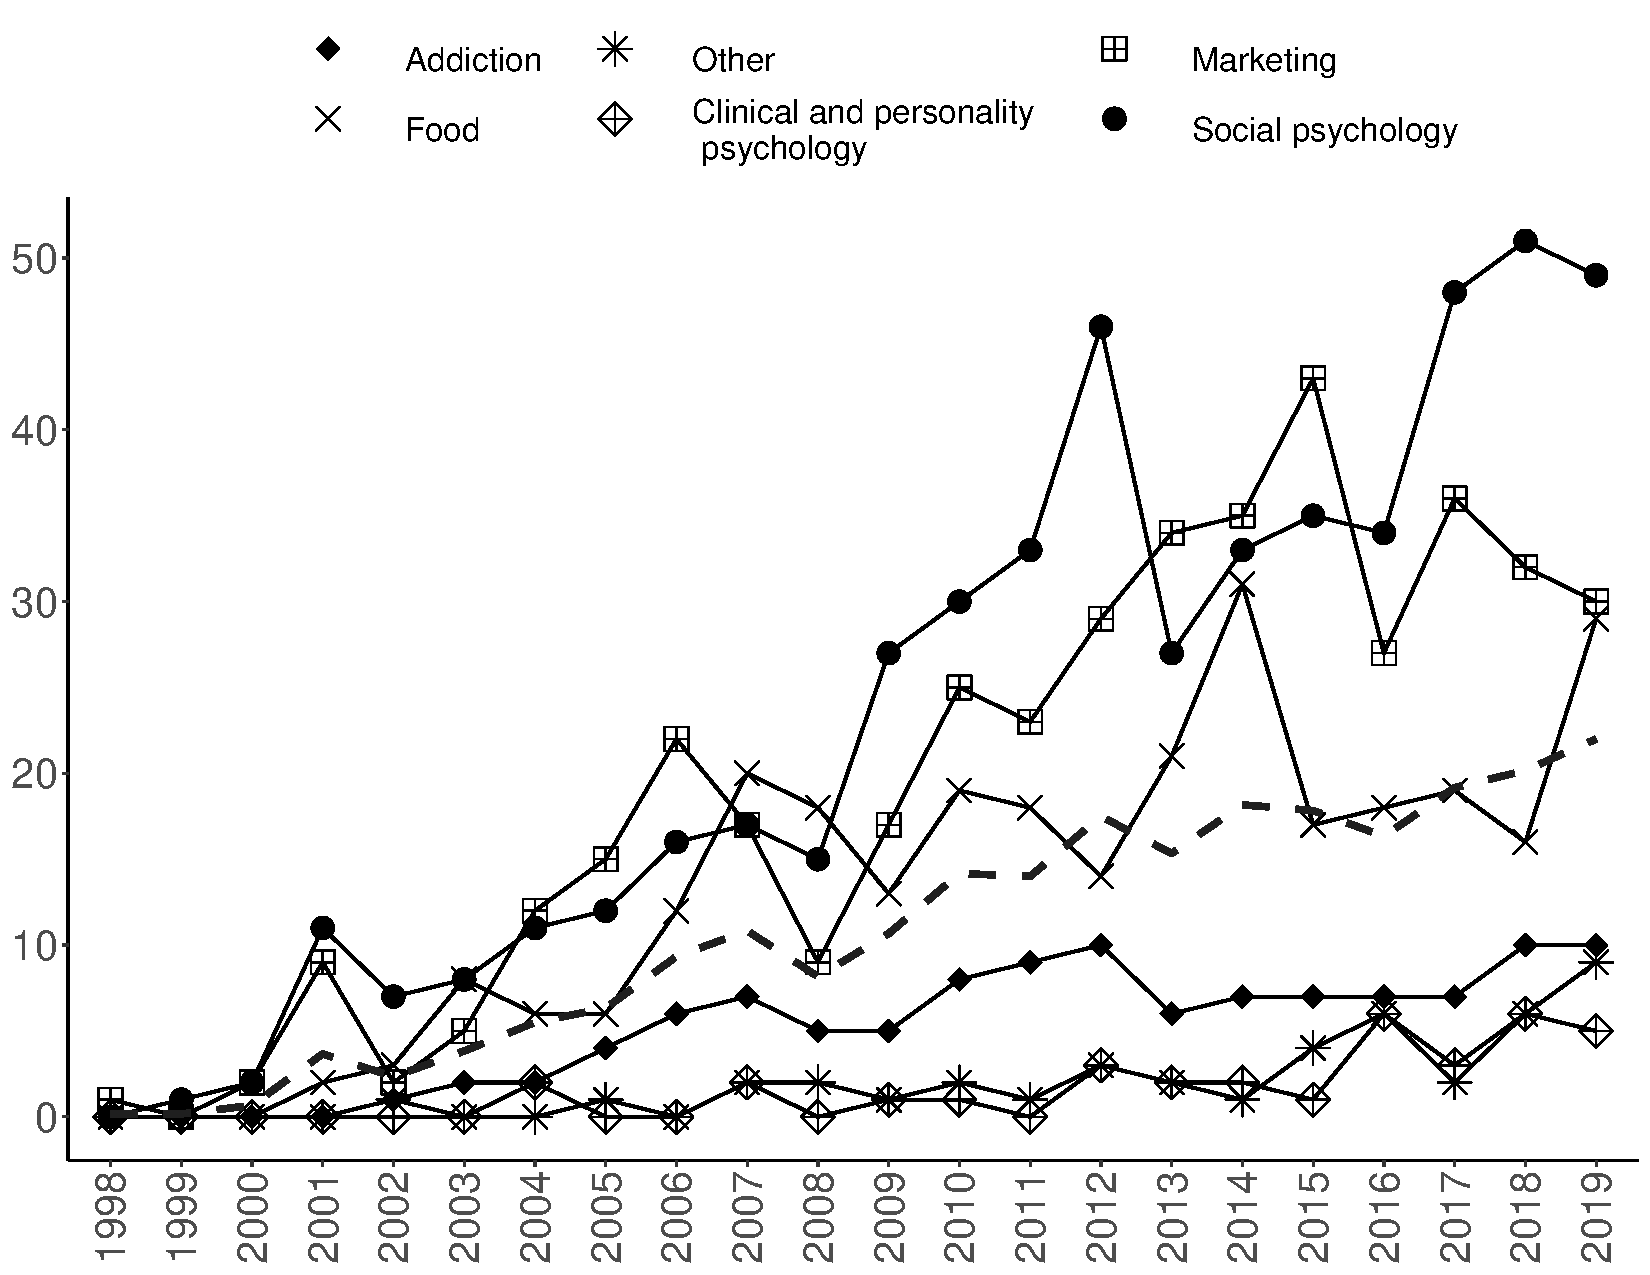
\includegraphics[width=.80\linewidth]{yearsIAT.pdf}
	\end{figure}
\end{frame}

\section[Altre misure]{Altre misure implicite}


\begin{frame}
	\onslide<1->
	\tikzoverlay (n1) at (1cm, 1cm){%
		\begin{minipage}{0.1\linewidth}
			\centering	
\includegraphics[width=\linewidth]{coca3.jpg}
		\end{minipage}
	}; %
	\onslide<1->
	\tikzoverlay (n2) at (7cm, 1cm){%
		\begin{minipage}{0.4\linewidth}
			\centering	
\includegraphics[width=0.25\linewidth]{pepsi3.jpg}
		\end{minipage}
	}; %
	\onslide<1->
	\tikzoverlay (n3) at (5cm, 0.5cm){%
		\begin{minipage}{0.4\linewidth}
			\huge \textbf{vs}
		\end{minipage}
	}; %	
	
	\onslide<2->
	
	\vspace{10mm}
	IAT $\rightarrow$ Misura \emph{comparativa} di quanto piace un oggetto rispetto al suo ``opposto''
	
	\vspace{5mm}
	\pause
	Problemi: 
	\begin{itemize}
		\item Non è sempre facile trovare un oggetto che sia effettivamente l'opposto rispetto all'oggetto di interesse 
		\vspace{2.5mm}
		\item La misura che si ottiene dell'oggetto di interesse in realtà dipende dalla categoria di contrasto che si è deciso di utilizzare! 
		\vspace{2.5mm}
		\item Ci sono casi in cui è più utile ottenere una misura ``assoluta'' rispetto a un oggetto di interesse 
	\end{itemize}

\end{frame}

\subsection{Single Category IAT}
\begin{frame}

\onslide<1->
\tikzoverlay (n1) at (10cm, 1.5cm){%
	\begin{minipage}{0.1\linewidth}
		\centering	
\includegraphics[width=\linewidth]{coca3.jpg}
	\end{minipage}
}; %


	Karpinski \& Steinman (2006):
		
	\begin{spacing}\Factor
		\begin{table}
				\centering
			\caption{SC-IAT}
			\begin{tabular}{c c c c}
				\hline
				Blocco	&	\# Trial	&	Tasto sinistro (E)	&	Tasto destro (I)	\\
				\hline
				1	&	24	&	Good + Coke	&	Bad	\\
				\textcolor<2->{unipd}{2}	&	\textcolor<2->{unipd}{72}	&	\textcolor<2->{unipd}{Good + Coke}	&	\textcolor<2->{unipd}{Bad}	\\
				3	&	24	&	Good 	&	Bad + Coke	\\
				\textcolor<3->{blu}{4}	&	\textcolor<3->{blu}{72}	&	\textcolor<3->{blu}{Good}	&	\textcolor<3->{blu}{Bad + Coke}	\\
				\hline
			\end{tabular}
		\end{table}
	\end{spacing}
	
	\begin{columns}
		\begin{column}{.50\linewidth}
			\centering
			\onslide<2->
			\textcolor{unipd}{Coke-Good condition}
		\end{column}
	
	\begin{column}{.50\linewidth}
		\onslide<3->
		\centering
		\textcolor{blu}{Coke-Bad condition}
	\end{column}
	\end{columns}

\vspace{5mm}
\onslide<4->
\begin{itemize}
	\item Response Time Window (rtw, solitamente a 1,500 ms)
	\item Feedback ad ogni risposta data
\end{itemize}


\end{frame}

\begin{frame}
	\begin{columns}
		\column{.5\linewidth}
		\centering{\textcolor{unipd}{Coke-Good}}
		\begin{figure}
			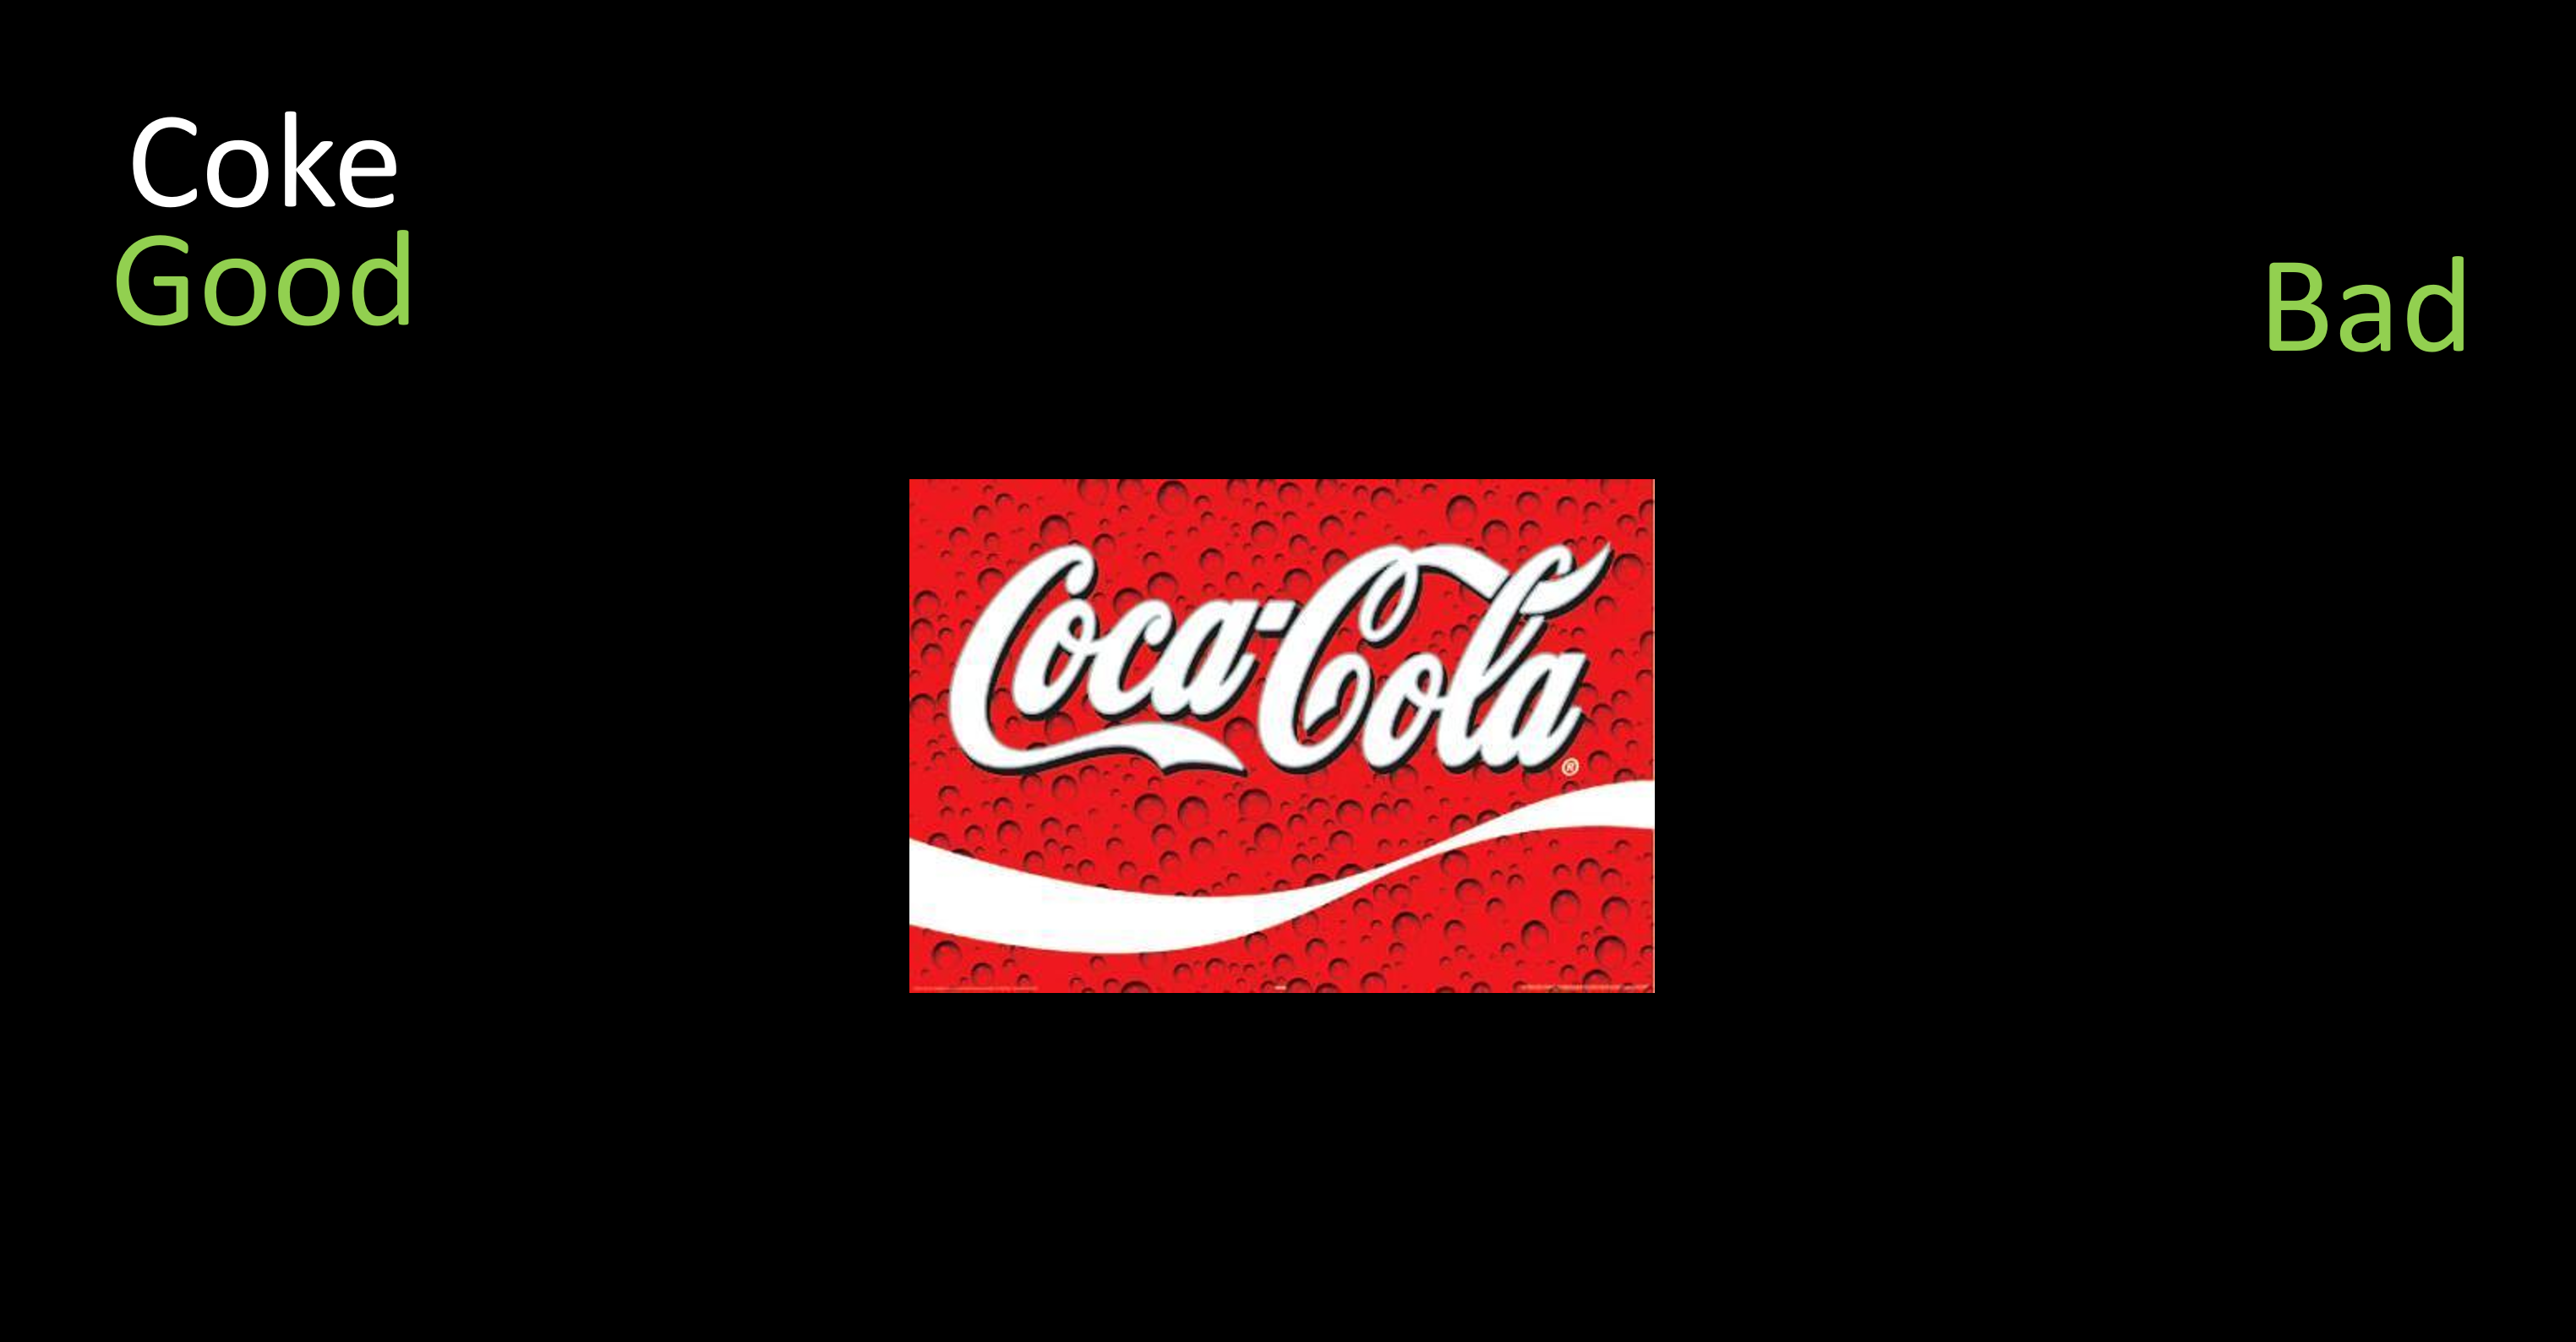
\includegraphics[width=\linewidth]{scGood.png}
		\end{figure}
		
		\column{.5\linewidth}
		\centering{\textcolor{blu}{Coke-Bad}}
		\begin{figure}
			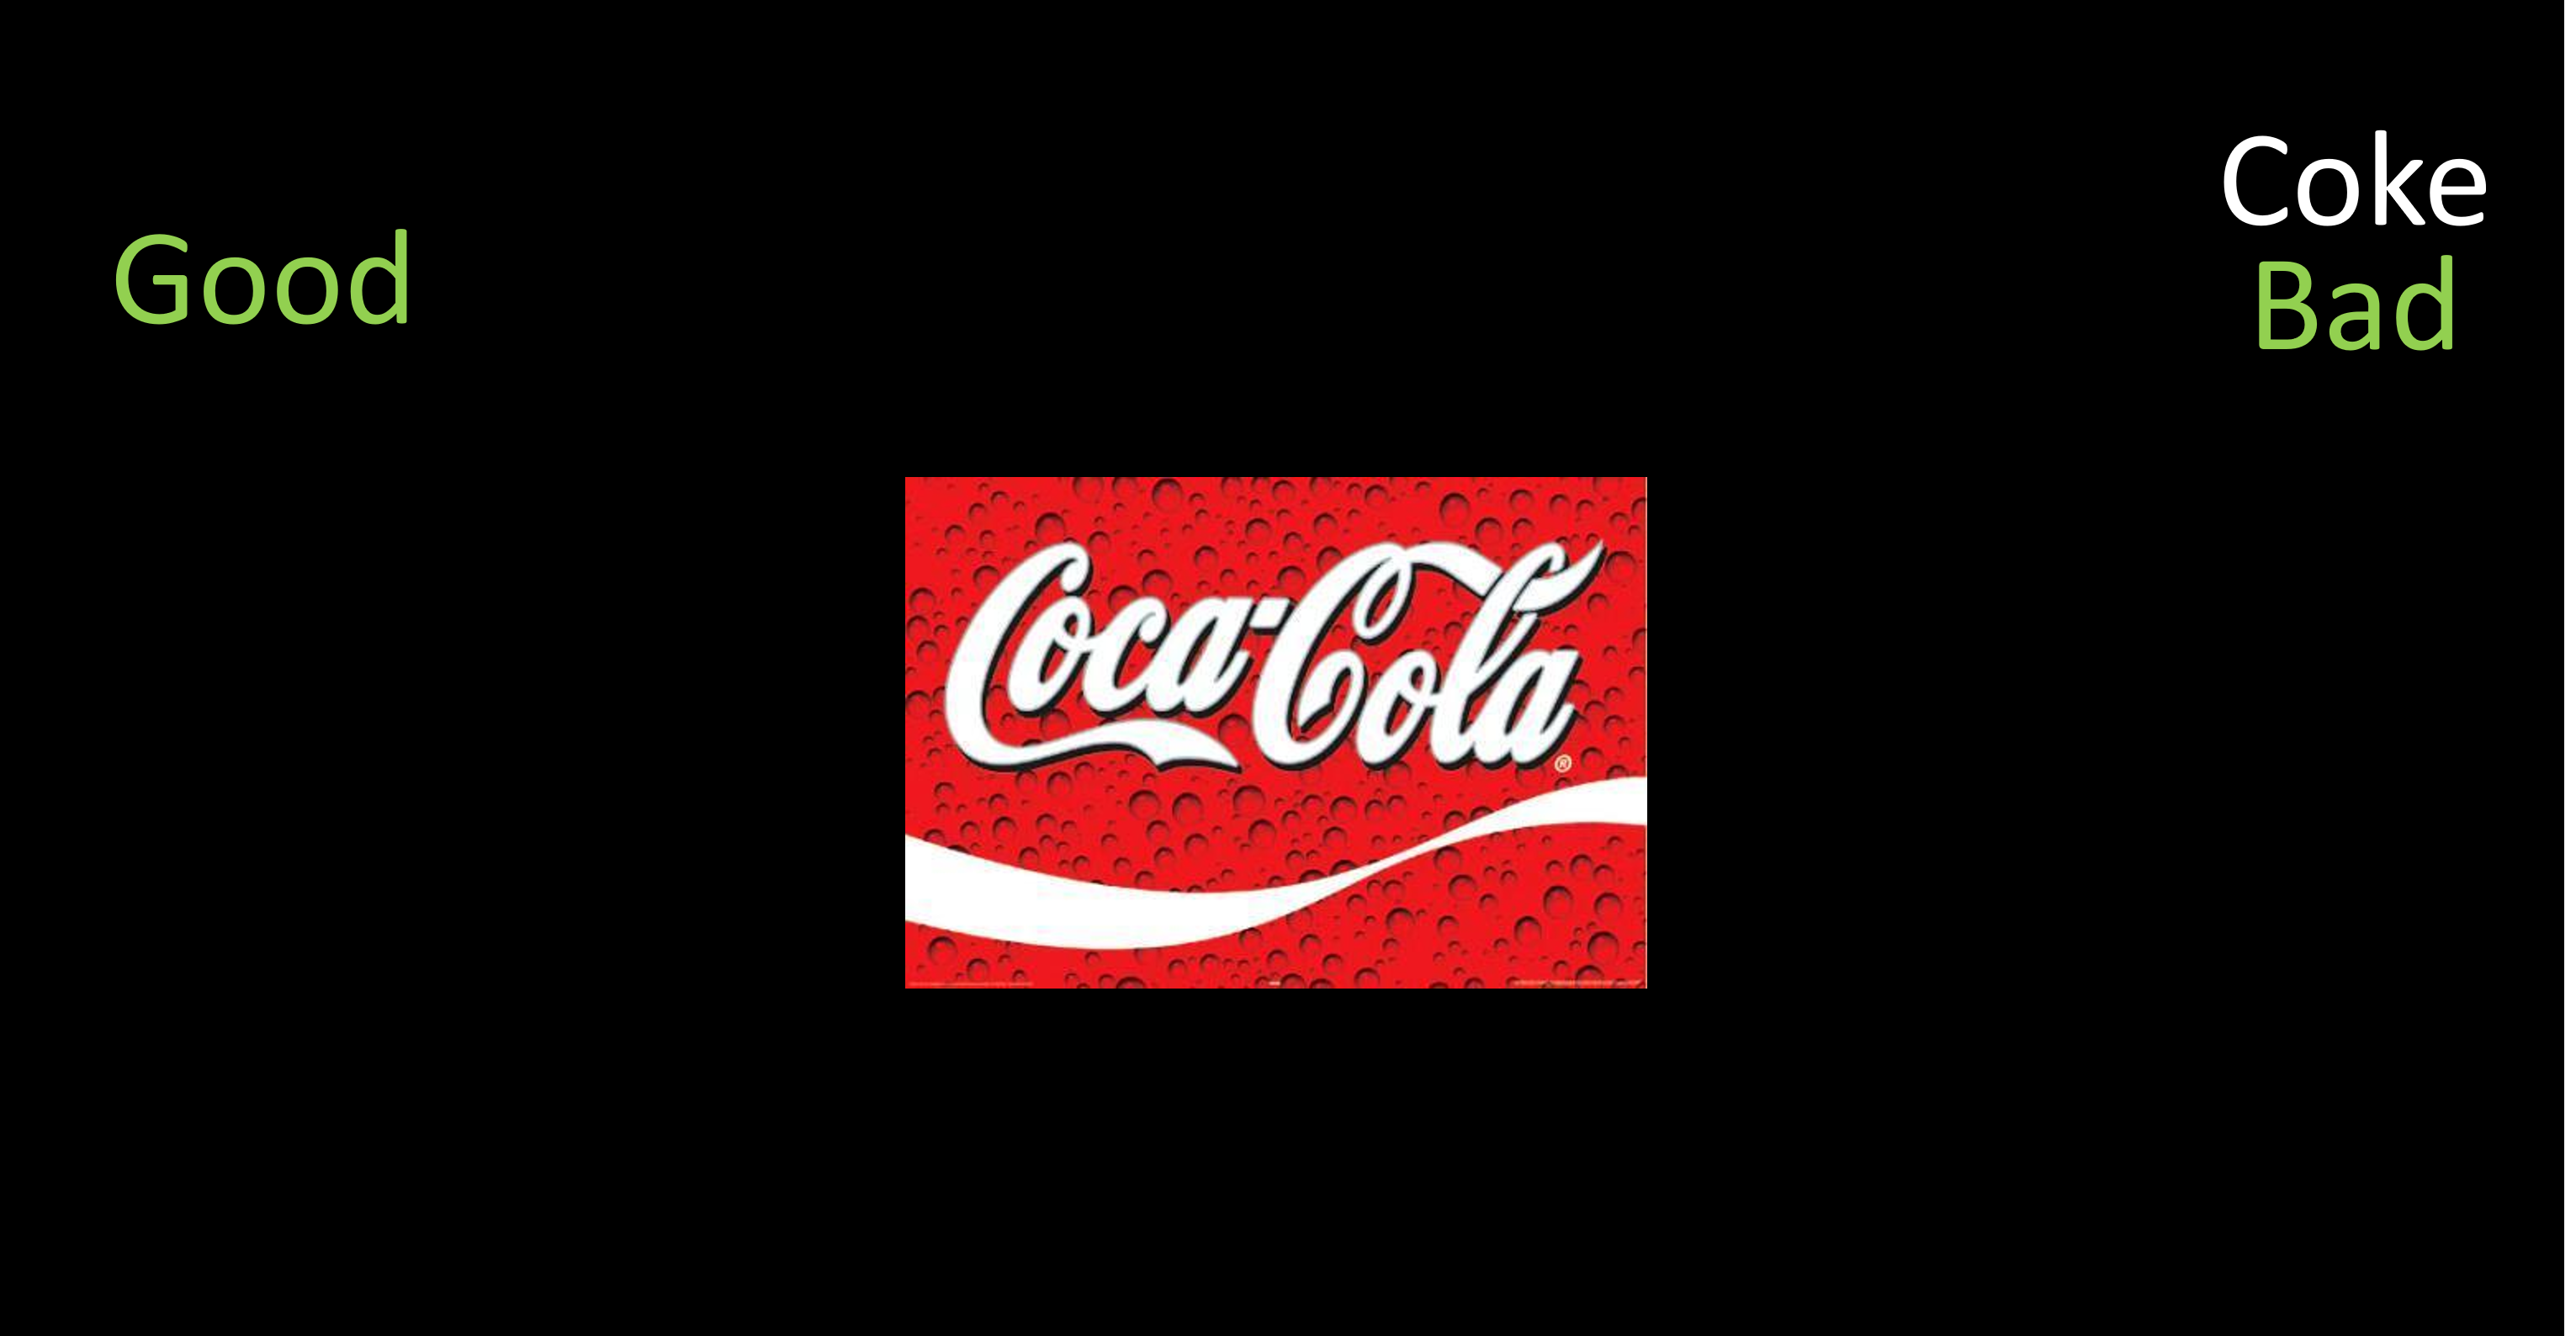
\includegraphics[width=\linewidth]{scBad.png}
		\end{figure}
	\end{columns}
	
\end{frame}


\begin{frame}{No Pepsi? No problem}
		\begin{columns}
		\column{.5\linewidth}
		\centering{\textcolor{unipd}{Pepsi-Good}}
		\begin{figure}
			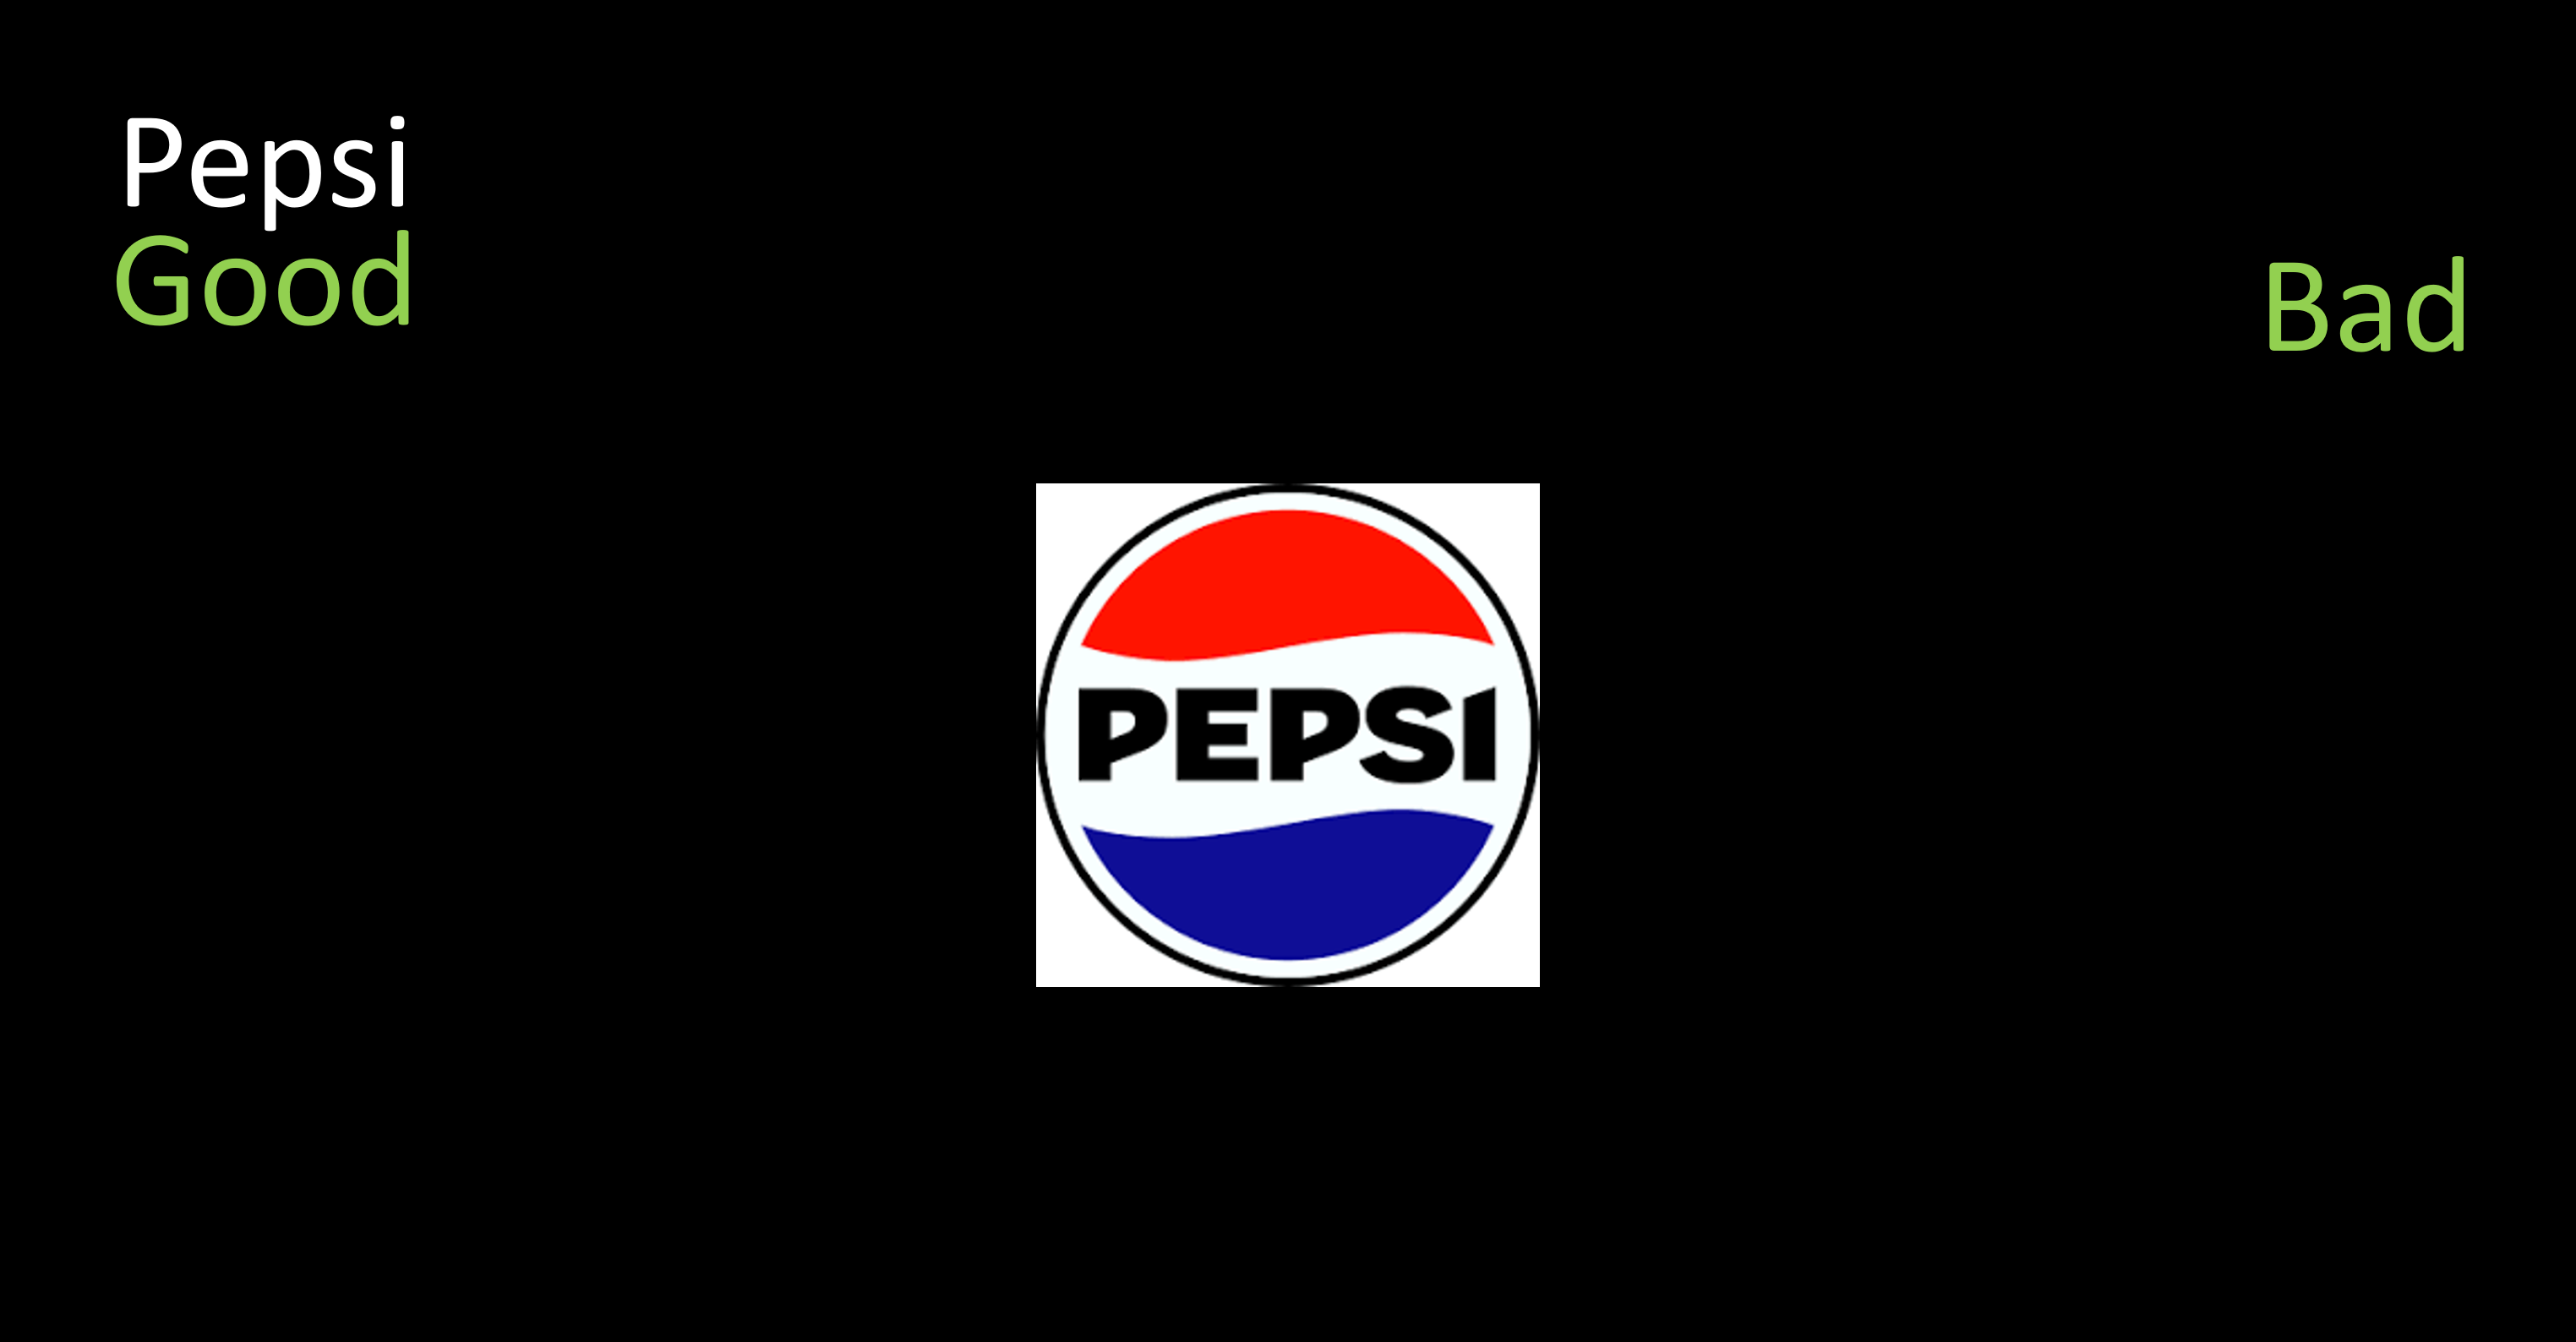
\includegraphics[width=\linewidth]{scPgood.png}
		\end{figure}
		
		\column{.5\linewidth}
		\centering{\textcolor{blu}{Pepsi-Bad}}
		\begin{figure}
			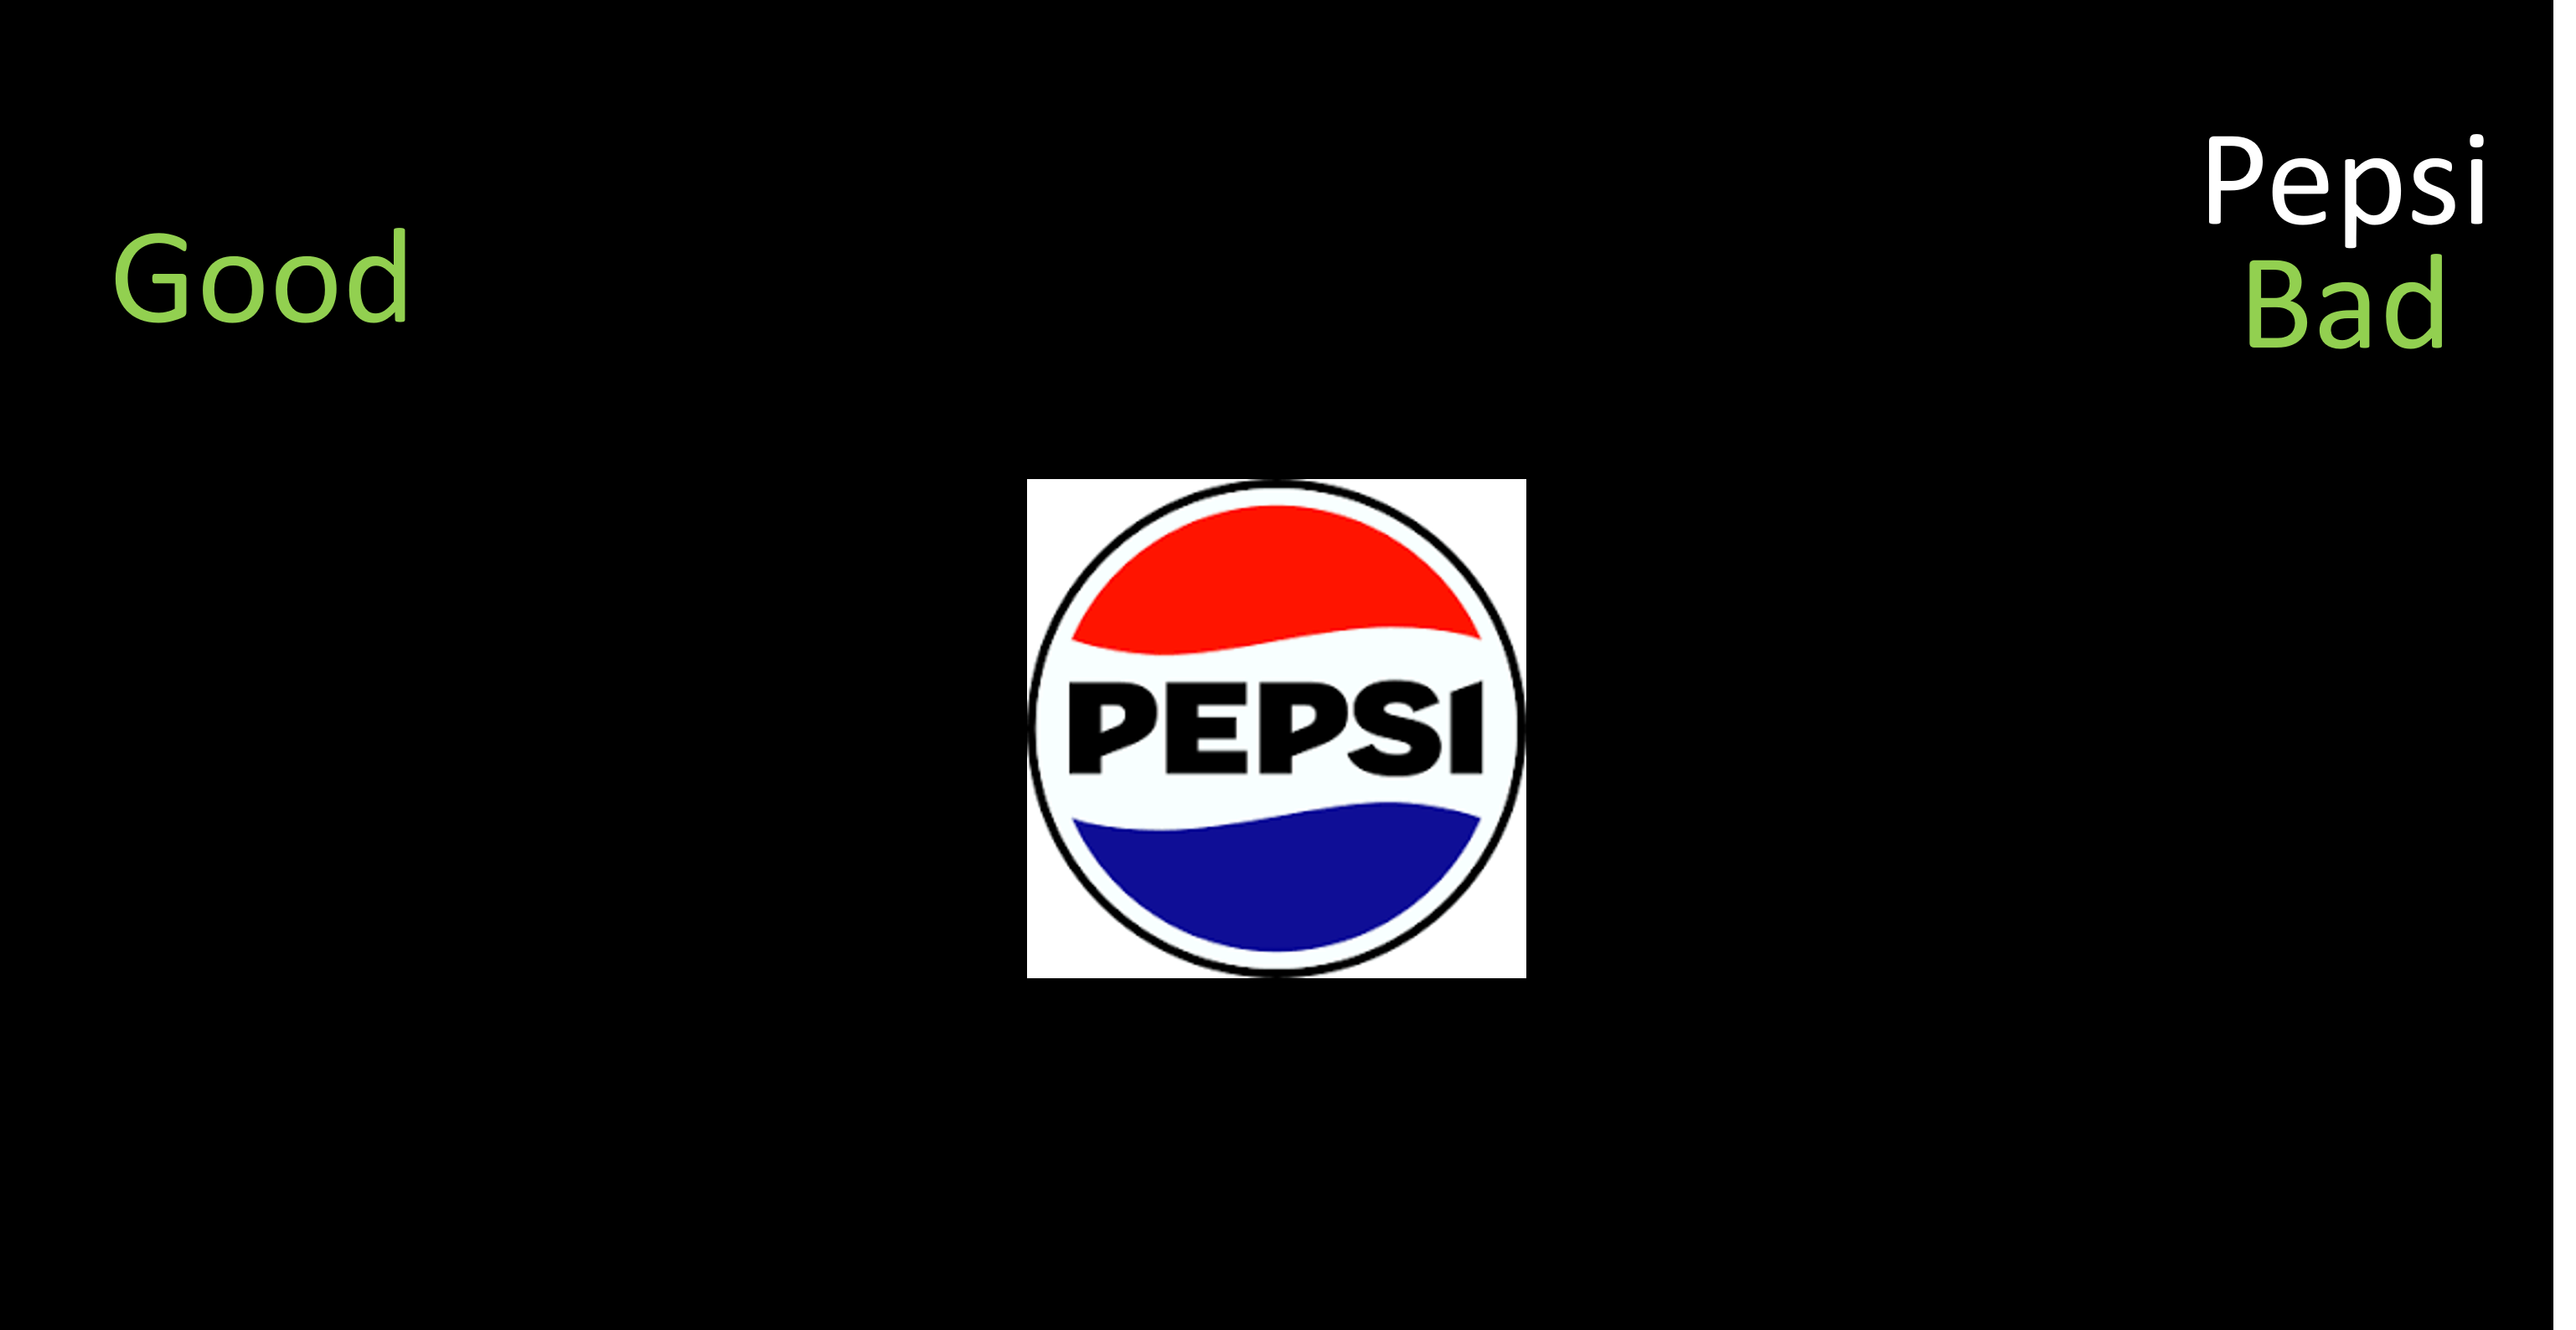
\includegraphics[width=\linewidth]{scPbad.png}
		\end{figure}
	\end{columns}
\end{frame}

\subsection*{Scoring}
\begin{frame}
	\vskip0pt plus 1filll
	\begin{equation*}
		D = \frac{M_{\mathrm{B2}} - M_{\mathrm{B4}}}{s_{\mathrm{B2, B4}}}
	\end{equation*}

\vspace{5mm}

\begin{itemize}
	\item Risposte $< 350$ms $ \rightarrow $ Eliminate
	\vspace{5mm}
	\item Risposte $> rtw$ $ \rightarrow $ Eliminate
	\vspace{5mm}
	\item Risposte errate $\rightarrow$ $M + 400$ms 
\end{itemize}
\vskip0pt plus 1filll

\color{template}\rule{0.30\linewidth}{0.5pt}\\
\color{black}
\scriptsize{Karpinski, A., \& Steinman, R. B. (2006). The single
	category implicit association test as a measure of
	implicit social cognition.\emph{ Journal of Personality and
	Social Psychology, 91}(1), 16–32. https://doi.org/10
	.1037/0022-3514.91.1.16}

\end{frame}

\subsection{Go/No-go association Task}
\begin{frame}
	Nosek \& Banaji (2001):
	
	
			\begin{table}
				\caption{GNAT}
				\begin{tabular}{c c c c }
					\hline
						Blocco	&	\# Trial	&	Signal (Spazio)	&	Noise (Niente)	\\
		\hline
		1	&	16	&	Good	&	Bad	\\
		2	&	16	&	Bad	&	Good	\\
		3	&	16	&	Fruit	&	Bugs	\\
		4	&	16	&	Bugs	&	Fruit	\\
		\hline
		\textcolor<2>{blu}{5}	&	\textcolor<2>{blu}{16}	&	\textcolor<2>{blu}{Good + Fruit}	&	\textcolor<2>{blu}{Bad + Bugs}	\\
		&	\textcolor<2>{blu}{60}	&	\textcolor<2>{blu}{Good + Fruit}	&	\textcolor<2>{blu}{Bad + Bugs}	\\
		\textcolor<2>{unipd}{6}	&	\textcolor<2>{unipd}{16}	&	\textcolor<2>{unipd}{Bad + Fruit}	&	\textcolor<2>{unipd}{Good + Bugs}	\\
		&	\textcolor<2>{unipd}{60}	&	\textcolor<2>{unipd}{Bad + Fruit}	&	\textcolor<2>{unipd}{Good + Bugs}	\\
		\hline
		\textcolor<3>{blu}{7}	&	\textcolor<3>{blu}{16}	&	\textcolor<3>{blu}{Good + Bugs}	&	\textcolor<3>{blu}{Bad + Fruit}	\\
		&	\textcolor<3>{blu}{60}	&	\textcolor<3>{blu}{Good + Bugs}	&	\textcolor<3>{blu}{Bad + Fruit}	\\
		\textcolor<3>{unipd}{8}	&	\textcolor<3>{unipd}{16}	&	\textcolor<3>{unipd}{Bad + Bugs}	&	\textcolor<3>{unipd}{Good + Fruit}	\\
		&	\textcolor<3>{unipd}{60}	&	\textcolor<3>{unipd}{Bad + Bugs}	&	\textcolor<3>{unipd}{Good + Fruit}	\\
		\hline
				\end{tabular}
			\end{table}


\end{frame}



	\begin{frame}
		\vskip0pt plus 1filll
		
		\begin{columns}
			\column{.5\linewidth}
			\centering{\large{\textbf{\textcolor{green}{GO}}}}
			\begin{figure}
				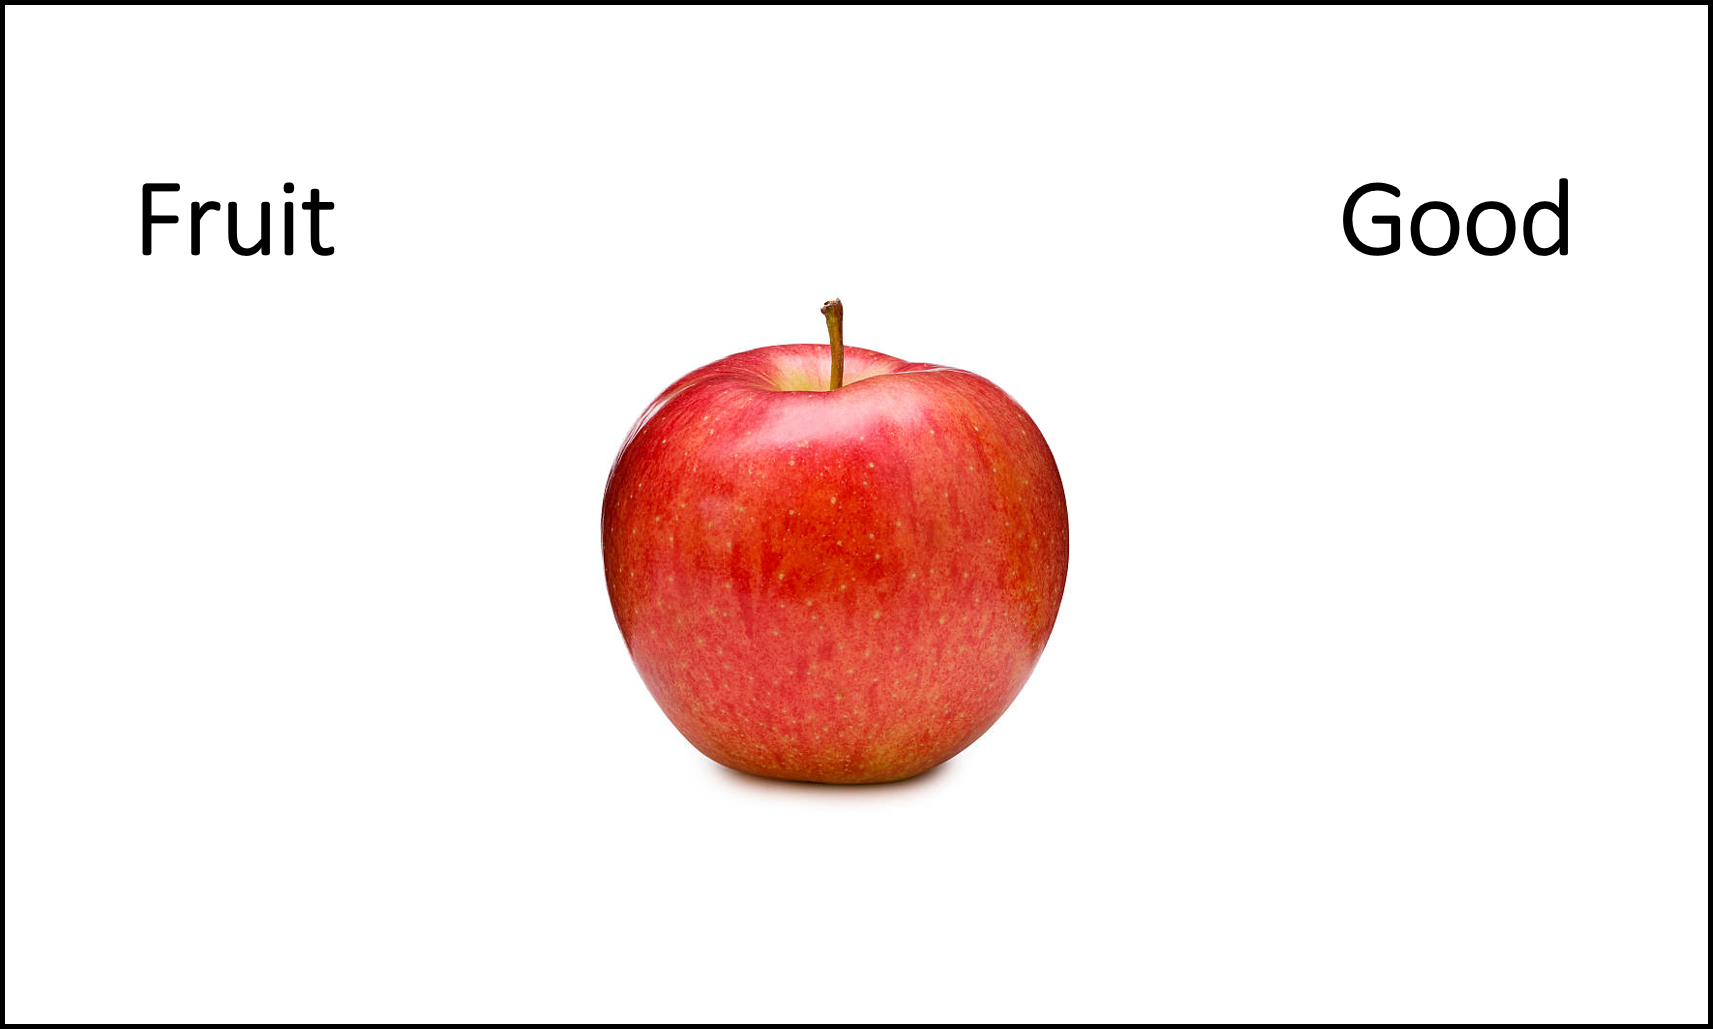
\includegraphics[width=\linewidth]{go.png}
			\end{figure}
			
			\column{.5\linewidth}
			\centering{\large{\textbf{\textcolor{unipd}{NO GO}}}}
			\begin{figure}
				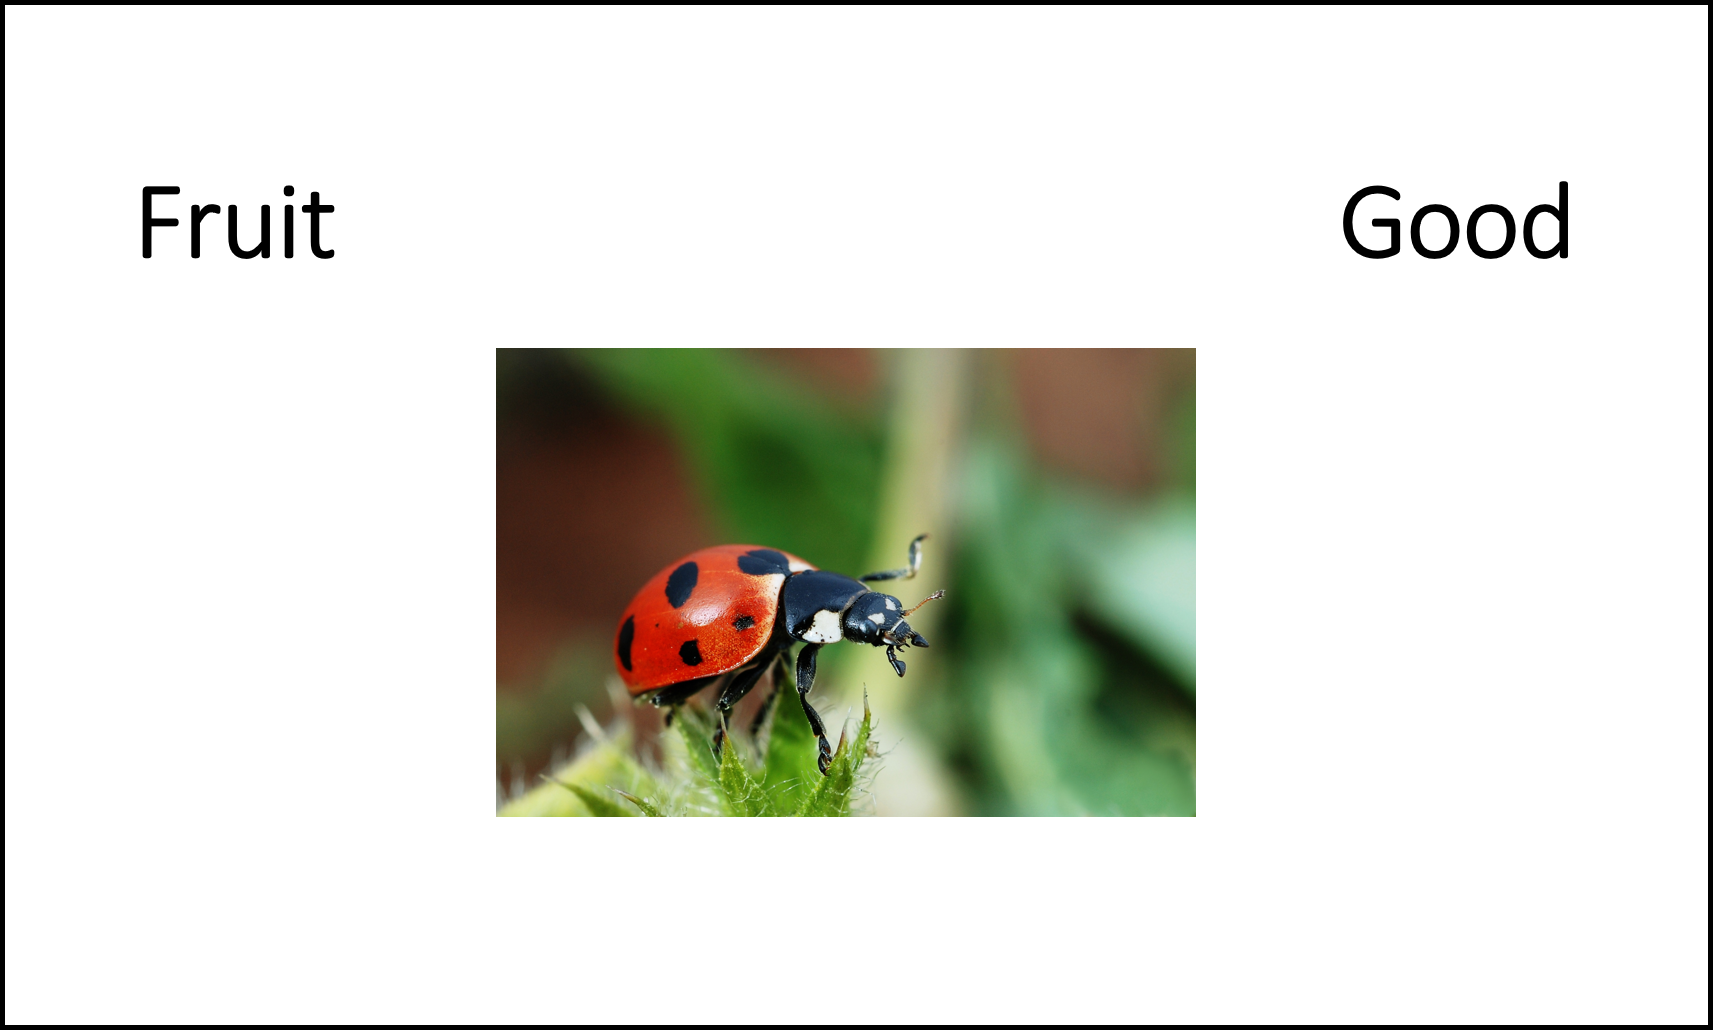
\includegraphics[width=\linewidth]{nogo.png}
			\end{figure}
		\end{columns}
	
	\vskip0pt plus 1filll
	
	
	\color{template}\rule{0.30\linewidth}{0.5pt}\\
	\color{black}
	
	\scriptsize{Nosek, B. A., \& Banaji, M. R. (2001). The go/no-go
		association task. \emph{Social Cognition, 19}(6), 625–666.
		Q21 https://doi.org/10.1521/soco.19.6.625.20886}
\end{frame}

\begin{frame}{Scoring}
	
$ d' $ (Green \& Swets, 1966): 

\vspace{5mm}

\begin{enumerate}
	\item Standardizzazione della proporzione di ``hits'' (risposte ``go'' in presenza del segnale)  
	\item Standardizzazione della proporzione di ``false alarms'' (risposte ``go'' in presenza di rumore)
	\item Differenza tra i due punteggi
\end{enumerate}
	
%	\vspace{5mm}
%	
%	Empty cells (no false alarms or misses) $\rightarrow$ $0.35/\mathrm{number \, of \, trials}$
\end{frame}

\subsection{Sorting Paired Features Task}
\begin{frame}
	\vskip0pt plus 1filll
	Bar-Anan et. al (2009):
	
	\begin{footnotesize}
			\begin{spacing}\Factor
			\begin{table}
				\centering
				\caption{SPF}
				\begin{tabular}{c c c c c c}
					\hline
					Blocks	&	Trials	&	Top-left	&	Top-right	&	Bottom-left	&	Bottom-right	\\
					\hline
					1	&	48	&	Dogs+Good	&	Dogs+Bad	&	Cats+Good	&	Cats+Bad	\\
					2	&	48	&	Dogs+Bad	&	Dogs+Good	&	Cats+Bad	&	Cats+Good	\\
					3	&	48	&	Cats+Bad	&	Cats+Good	&	Dogs+Bad	&	Dogs+Good	\\
					4	&	48	&	Cats+Good	&	Cats+Bad	&	Dogs+Good	&	Dogs+Bad	\\
					\hline
					
				\end{tabular}
			\end{table}
		\end{spacing}
	\end{footnotesize}

\vspace{3mm}

Viene associata una chiave di risposta della tastiera ad ognuno dei possibili pairing 

\vskip0pt plus 1filll

\color{template}\rule{0.30\linewidth}{0.5pt}\\
\color{black}
\scriptsize{Bar-Anan, Y., Nosek, B. A., \& Vianello, M. (2009).
	The sorting paired features task: A measure of
	association strengths. \emph{Experimental Psychology,
		56}(5), 329–343. https://doi.org/10.1027/1618-3169.
	56.5.329}
\end{frame}

\begin{frame}
			\begin{columns}
		\column{.5\linewidth}
		\centering{\large{Correct key: M}}
		\begin{figure}
			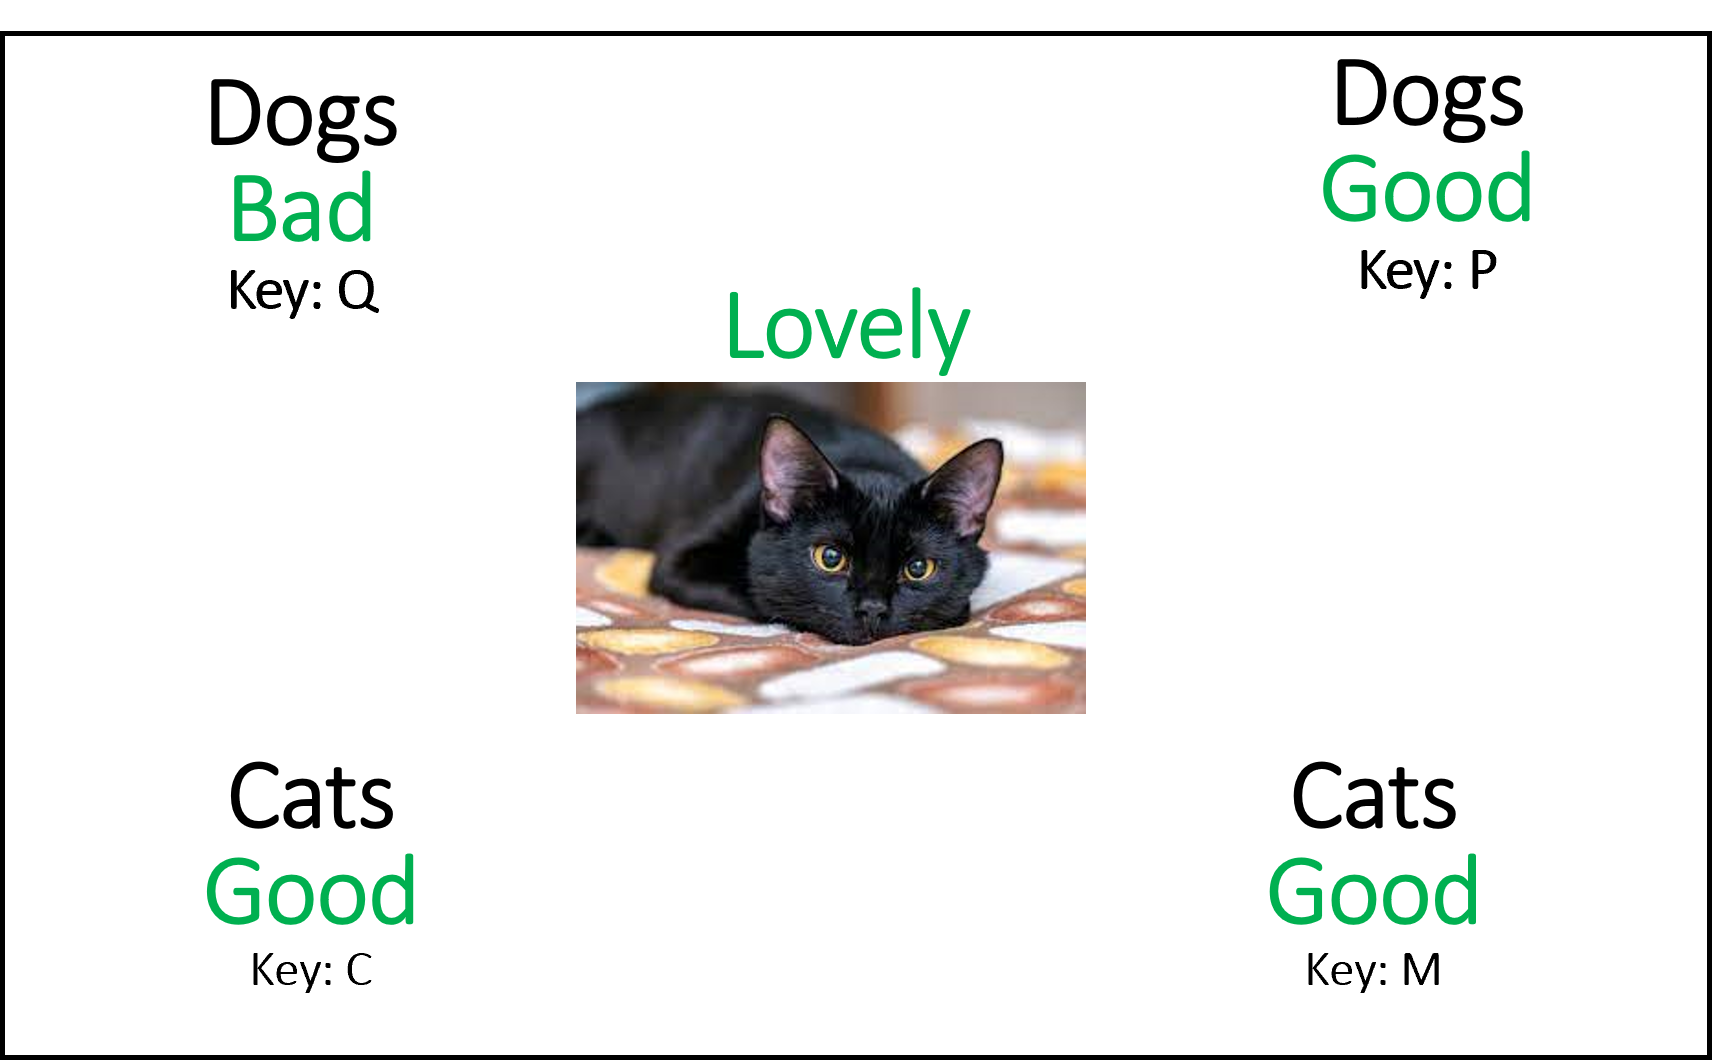
\includegraphics[width=\linewidth]{spf1.png}
		\end{figure}
		
		\column{.5\linewidth}
		\centering{\large{\large{Correct key: P}}}
		\begin{figure}
			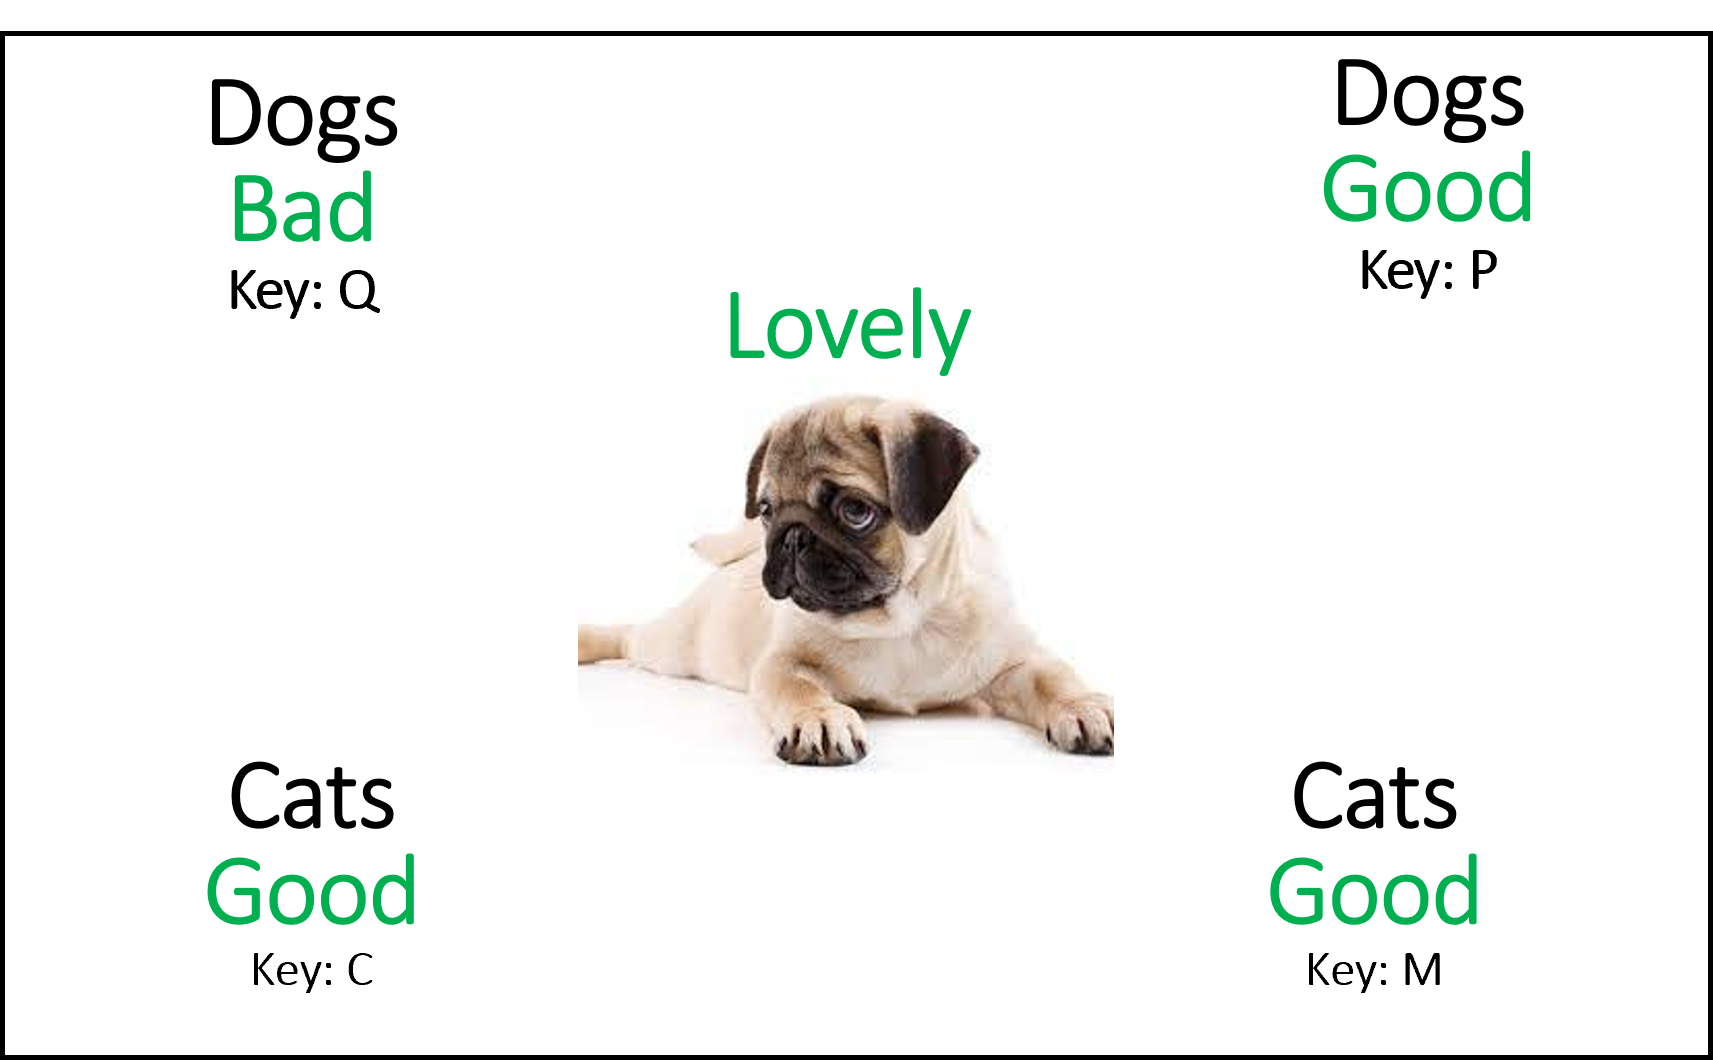
\includegraphics[width=\linewidth]{spf2.png}
		\end{figure}
	\end{columns}
\end{frame}



\section[Make it easy]{The easy way}

\begin{frame}
	%	\begin{spacing}\Factor
	\begin{table}[th!]
		\centering
		\begin{tabular}{llll}
			\hline
			\emph{D-score} & Error inflation & Delete trials $<$ 400 ms\\\hline
			\emph{D}1 & Built-in correction & No \\
			\emph{D}2 & Built-in correction & Yes \\
			\emph{D}3 & \emph{M} (correct responses) + 2\emph{sd} & No\\
			\emph{D}4 & \emph{M} (correct responses) + 600 ms & No \\
			\emph{D}5 & \emph{M} (correct responses) + 2\emph{sd} & Yes\\
			\emph{D}6 & \emph{M} (correct responses) + 600 ms & Yes \\\hline
		\end{tabular}
	
	\end{table}
	\begin{itemize}
		\item[\large{\Sadey}] Few Open source alternatives
		\item[\large{\Sadey}] Utterly complicated to use
		\item[\large{\Sadey}] No clear information on the algorithm they compute
		\item[\large{\Sadey}] No graphical representation of the results
	\end{itemize}
	
	\vspace{3mm}
	\pause
	\begin{tabular}{l p{9cm}}
		{
\includegraphics[height=5ex]{emoji.png}} & Something Open Source, able to compute multiple scores, and to provide nice graphical representations\\
	\end{tabular}

\end{frame}

\begin{frame}{Make it easy \& Clear}
	\href{https://cran.r-project.org/web/packages/implicitMeasures/index.html}{\texttt{implicitMeasures} package} DOI:\href{https://joss.theoj.org/papers/10.21105/joss.02394}{10.21105/joss.02394} : 
	
	\vspace{2mm}
	\begin{small}
		\begin{tabular}{p{2.3cm}p{8cm}}
			\hline
			Function & Description \\
			\hline
			\texttt{clean\_iat()} & Prepare and clean IAT data\\
			\texttt{clean\_sciat()} & Prepare and clean SC-IAT data\\
			\texttt{compute\_iat()} & Compute IAT \emph{D-score}\\
			\texttt{compute\_sciat()} & Compute SC-IAT \emph{D-score} \\
			\texttt{descript\_d()} & Descriptive table of \emph{D-score}s (even in \LaTeX) \\  
			\texttt{d\_density()} & Plot IAT or SC-IAT scores (distribution)\\
			\texttt{d\_point()} & Plot either IAT or SC-IAT scores (points)\\
			\texttt{IAT\_rel()} & IAT reliability\\
			\texttt{multi\_dsciat()} & Plot SC-IATs scores\\
			\texttt{multi\_dscore()} & Compute and plot multiple \emph{D-score}s\\
			\texttt{raw\_data()} & Dataset with one IAT and two SC-IATs\\
			\hline
		\end{tabular}
	\end{small}
	
	\begin{small}
		\begin{itemize}
			\item \href{https://cran.r-project.org/web/packages/implicitMeasures/vignettes/implicitMeasures.html}{\textcolor{blue}{implicitMeasures}}: Introduction to IAT, SC-IAT, and \emph{D score}s.
			\item \href{https://cran.r-project.org/web/packages/implicitMeasures/vignettes/IAT-example.html}{\textcolor{blue}{IAT-example}}: Package illustration on IAT data
			\item \href{https://cran.r-project.org/web/packages/implicitMeasures/vignettes/SC-IAT-example.html}{\textcolor{blue}{SC-IAT-example}}: Package illustration on SC-IAT data
		\end{itemize}
	\end{small}
\end{frame}

\begin{frame}{Make it even easier}
	\begin{center}
		\href{http://fisppa.psy.unipd.it/DscoreApp/}{
\includegraphics[width=0.4\linewidth]{AppLogo.png}}
	\end{center}
	\vspace{5mm}
	\color{black}
	Source code on \href{https://github.com/OttaviaE/DscoreApp}{\textcolor{blue}{GitHub}}	
	
	\vspace{3mm}
	DOI: \href{https://www.frontiersin.org/articles/10.3389/fpsyg.2019.02938/full}{10.3389/fpsyg.2019.02938}
\end{frame}

\end{document}
